\section{Ancillary Measurements}
The entrance face of the LXe calorimeter consists of 4092 MPPCs
arranged in a grid structure containing 93 rows in the $\phi$ direction.  
A row consists of 44 MPPCs placed along $Z$ direction, divided equally in two
PCB\footnote{Printed Circuit Board} strips on the upstream and
downstream side of the calorimeter \cite{megdesign}.  The PCB strips
are mounted with spacer materials on four CFRP\footnote{Carbon Fiber
Reinforced Polymer} plates, each containing 23-24 strips and attached
to the inner face of the cryostat at different $\phi$ locations.  The
in-situ position and alignment of the MPPCs and its installation
assembly is verified in the following sections.

\subsection{ Spacing in Z and $\phi$}
The photodetectors are manufactured and assembled in lattice formation
to high precision, which can be used for validation of the X-ray
scanning technique and calculate its resolution.  A change in the
spacing can also reveal the effect of thermal cooling as well as
installation errors.  The spacing between individual MPPC pairs as
well as mean spacing between adjacent MPPC is calculated per PCB strip
(row-wise) along Z and per cfrp plate (column-wise) along \phis. 

Table \ref{tab:oddeven} shows spacing between individual MPPC pairs separated
into two groups which include alternate pairs along columns for Z measurement,
and rows for $\phi$ measurement.  Nominally we expect the spacing to be equal in
the two groups; the data shows the spacing in Z coordinate differs by 0.88~mm
and 0.74~mrad in the $\phi$ coordinate.  The average spacing over the scanned
region (shown in table \ref{tab:avgspacing}), however, is consistent with
expectation after accounting for thermal cooling.  
This implies a systematic shift or miscalculated position 
of one set of every other MPPC by 0.22~mm (0.18 mrad), and the oppposite 
shift for the complementary set, such there is not net displacement over the entire
row or column. 


The source of this discrepancy is not known.
Two possible causes were investigasted that could introduce observed 
systematic shifts in reconstructed MPPC positions with the periodicty of 
$\sim$30 mm, or two MPPC widths: X-ray corrections and trigger bias.
Although inaccurate corrections to the X-ray position can introduce the magnitude of 
displacement in MPPC position observed the periodicity of the corrections
does not match that of the observed effect; Z corrections have a period of 
100~mm while $\phi$ corrections are monotonic.
Similarly, studies of the effect of trigger configuration on the reconstructed position 
were not able to replicate this effect. 


As the scale of the systematic shift is small compared to the overall
X-ray measurement uncertainty as well as the precision goals of the
MEG experiment, it is expected to have minimal effect on the photon
position resolution.  We estimate this effect on photon reconstrution
using MC simulation.  A photon interaction is simulated at
normal distance equivalent to one radiation length
($\lambda_{LXe}\approx$ 2.75 cm) over a two dimensional surface
consisting of (20 $\times$ 20) photodetector array.  The dimensions and
spacing of the photodetectors are identical to the MPPC 
in the LXe calorimeter.  The isotropic distribution of photons generated as a
result is recorded by the photodetector array. The signal in each
photodetector is proportional to the solid angle subtended to the
interaction point, and detection efficiency determined by the photon
incident angle, measured in standalone tests.  
Each event is simulated with an interaction point
chosen randomly in a 30$\times$30~mm$^2$ region equivalent to two MPPC
widths, and reconstructed twice, with nominal and systematically
shifted photodetector positions by 0.22~mm.  The photon position is
reconstructed using weighted mean of the signal recorded in the
photodetectors.
The results show no mean displacement, while the photo 
position resolution is degraded by 0.08~mm in the 
measurement plane.

The mean distance between adjacent MPPCs is calculated using only the
measurements at the end of the row or column.  The precision of the
measurement is improved as a result compared to the pair-wise spacing
by  one (two) order of magnitude in Z ($\phi$).  In the Z coordinate,
the mean distance is calculated for each PCB strip as well as for the
half-strips (US and DS) connected at the center.  Similarly in the
$\phi$ coordinate, the mean distance is calculated within individual
cfrp plates and overall.  The mean and standard deviation of the
calculated mean distance in Z and $\phi$  show a regular grid
structure with no deformation in the scanned region (table
\ref{tab:avgspacing}).

The effect of thermal cooling is seen in Z with the mean distance
15.08~mm  or 30~\micron contraction between adjacent MPPCs. The mean
distance in $\phi$ is dependent on the X-coordinate of the
semi-cylindrical LXe calorimeter whose center is nominally aligned
with the center of the X-ray scanning device.  During the X-ray survey
the calorimeter was off-center, shifted towards the X-ray device by
3.85~mm increasing the mean angular spacing seen in the data.  The
following sections detail the qualitative use of X-ray data to measure
thermal contraction and 3D MPPC location.

\begin{table}
\begin{tabular}{ccccc}
 & $Z_{n} - Z_{n-1}$ &Std. Dev.& $\phi_{n} - \phi_{n-1}$ & Std. Dev. \\
 & [mm] &[mm]& [mrad]& [mrad]\\
\hline
Odd  $n$ & 15.69 & 0.49 & 24.12 & 0.54 \\ 
Even $n$ & 14.57 & 0.57 & 23.38 & 0.70 \\ 
%Nominal  & 15.1  &      & 23.55 & \\
\end{tabular}
\caption{Mean Z and $\phi$ spacing calculated for Odd-Even and Even-Odd
combination  of adjacent MPPCs.}
\label{tab:oddeven}
\end{table}

\begin{table}
\begin{tabular}{clc}
   & Z [mm] &Std. Dev. [mm] \\
\hline
US     & 15.091(32)& 0.127  \\
DS     & 15.101(49)& 0.164  \\
All    & 15.081(8) & 0.061  \\
Nominal& 15.1      &
\end{tabular}

\begin{tabular}{clc}
   & $\phi$ [mrad] &Std. Dev. [mrad] \\
\hline
cfrp 1     & 23.733(13)& 0.032  \\
cfrp 2     & 23.716(15)& 0.055  \\
cfrp 3     & 23.689(12)& 0.035  \\
cfrp 4     & 23.727(11)& 0.037  \\
All        & 23.725(2) & 0.008  \\
Nominal    & 23.55 &     
\end{tabular}
\label{tab:avgspacing}
\caption{Mean distance between adjacent MPPC calculated over the entire row (Z) or 
column ($\phi$). Upstream (US) and downstream (DS) parts of each PCB strip, and
individual cfrp plates are calculated separately, and altogether.}
\end{table}

\subsection {R coordinate calculation and 
coefficient of thermal expansion}
The radial coordinate not directly measured in the X-ray scan is
calculated using information from the FARO scan of the photodetectors.
The FARO scan provides highly precise 3D coordinates
($\sigma_{|\vec{x}|}$ = 200 \micron) of a subset of photodetectors
(10\%) measured at room temperature. To determine the position of
every photodetector, these measurements are interpolated by fitting
the 3D surface formed by the photodetectors. The radial coordinate and
center are calculted first with a cylindrical fit function, followed
by z,$\phi$ coordinates fitted to a regularly spaced grid in z-$\phi$
plane allowing for small rotations in the plane.  Each cfrp plate is
fitted independently since the curvature varies slightly between
individual plates and the overall curvature of the calorimeter.  


The interpolated photodetector locations from FARO
and X-ray scans are fitted with degrees of freedom to account for
global translational motion, extrinsic rotation centered in the MEG
coordinate  system, and scale factor for thermal contraction. 
The FARO coordinate is transformed using the equation
\begin{align}
\vec{x}_{FARO}^{'} = (1-s)R(\alpha,\beta,\gamma)\vec{x}_{FARO} +
\vec{x}_{offset},  
\end{align}
where $s$ is the scale of thermal contraction, $R$ is the rotation
matrix  and $\vec{x}_{offset}$ is the linear offset. 
The fit parameter values are extracted by minimizing the following function
\begin {align}
\chi^2 = 
\sum\limits_{i}^{N_{MPPC}} \frac{(Z_{i}^{Xray}-Z_{i,FARO}^{'})^2}{\sigma_{Z_{i}}^2} 
+ 
\frac{(\phi_{i}^{Xray}-\phi_{i,FARO}^{'})^2}{\sigma_{\phi_i}^2},
\end{align}
where $\sigma_{Z_i}$ and $\sigma_{\phi_i}$ include the resolution
of X-ray and FARO measurements
added in quadrature: 
$\sigma^{FARO}$ = 0.14~mm (0.25~mrad), 
$\sigma^{Xray}$ = 0.40~mm (0.56~mrad),
calculated from adjacent MPPC spacing described above.


The radial values from the FARO measurement are transformed using
fitted parameters to calculate radial coordinate of each
photodetector.  The uncertainty is calculated using linear error
propagation and corresponds to change in the main result due to one
standard deviation variation in the parameters taking correlations
into account.  The results in table \ref{tab:radius} shown mean radius
648.7 and 644.9~mm,and mean error 0.16 and 0.27~mm respectively in the
two scans(figure~\ref{fig:radiuscalculation}).  The radial coordinate
change of 3.8~mm between the two scans is consistent with the shift of
equal magnitude (3.85$\pm$0.1~mm) in the X-coordinate of the LXe
calorimeter in the same period.  A $\phi$ dependent change in the
radial coordinate is seen in 2018 data compared to the previous year's
data due to the calorimeter center offset with respect to the X-ray
device in 2018.



The thermal expansion coefficient is calculated as
\begin{align}
 s= \alpha_t \, \Delta T,
\end{align}
where s is the scale of thermal contraction, $\alpha_t$ is coefficient
of thermal expansion and $\Delta T$ is the change in temperature. 
Using $\Delta T$ ( = 123$\pm$10 K) 
between FARO survey performed at room temperature
(293 K) and X-ray survey performed at LXe temperature (170 K)
the thermal coefficient is calculated in the
two X-ray surveys (table \ref{tab:thermalcoefficient}).
\begin{table}[h]
\begin{tabular}{ccc}
Scan Period & $s$ & $\alpha_t \,\, [\mathrm{ppm K}^{-1}]$\\
\hline
2017 & 0.0015(1) & 11.7$\pm$1.9 \\
2018 & 0.0017(4) & 13.1$\pm$3.5 
\end{tabular}
\caption{Fitted scaling parameter ($s$) and the calculated thermal 
expansion coefficient.}
\label{tab:thermalcoefficient}
\end{table}
The theoretical value of $\alpha_t$ for the
detectaor material is 16$\pm$1 ppmK$^{-1}$.

The photodetector positions measured from the two X-ray surveys are
compared using the same fitting procedure to verify the stability 
of the photodetector ensemble.
The motion between the two
must be understood relative to the motion of the LXe calorimeter
position which has also moved between the two surveys.  Multiple
positions on the external surface of the calorimeter were optically
surveyed before each X-ray survey to record its location.  
Overall the motion of the calorimeter is replicated well 
by the photodetectors (table \ref{tab:xray2017vs2018}),
characterized by small angular rotations, and 
large displacement along X-axis seen in both data. 

\begin{table}[h] 
\begin{tabular}{rrr} 
Fit Paramter & Optical Survey &
X-ray Survey \\ 
\hline 
dx [mm] & 3.85 (7)      & 3.83 (6) \\ 
dy [mm] & -1.2 (2)      & -0.7 (2) \\ 
dz [mm] & 0.1 (2)       & -0.9 (2) \\ 
rx [mrad] & -0.0 (1)    & -0.1 (1) \\ 
ry [mrad] & -0.2 (2)    & 0.2 (4)    \\ 
rz [mrad] & -0.9 (2)    &  -0.3 (3)  
%%lxe
%%  1  rx          -4.98974e-05   1.12590e-04   1.81586e-08  -5.11285e-04
%%   2  ry          -2.46074e-04   1.69744e-04   8.54602e-09   1.55717e-02
%%   3  rz          -8.69646e-04   1.75347e-04   8.56504e-09   2.63737e-03
%%   4  dx           3.85602e+00   7.18101e-02   3.55683e-08   1.44061e-03
%%   5  dy          -1.18210e+00   2.30683e-01   3.55680e-08   7.98124e-04
%%   6  dz           1.45227e-01   2.24210e-01   3.55680e-08   3.00940e-03
%%
%%xray
%%   1  rx          -9.03902e-05   1.03847e-04   2.07576e-07  -4.03030e-03
%%   2  ry           1.73869e-04   3.56954e-04   1.50140e-07   8.05430e-03
%%   3  rz          -3.49186e-04   3.02230e-04   1.19763e-07  -2.19844e-02
%%   4  dx           3.83337e+00   6.64374e-02   4.16831e-07   2.82117e-03
%%   5  dy          -6.77152e-01   2.39740e-01   3.01004e-07   9.43571e-03
%%   6  dz          -9.02411e-01   1.90330e-01   2.49133e-07   5.52444e-03
\end{tabular}
\caption{Fit parameters denoting change in position of the calorimeter
(from optical survey) and the photodetector position (X-ray survey),
between the two data-taking periods, 2017 and 2018.}
\label{tab:xray2017vs2018} \end{table}



\begin{table}
\begin{tabular}{ccccc}
 & $R^{2017}$ & $\sigma_R^{2017}$ & $R^{2018}$  & $\sigma_R^{2018}$  \\
\hline
cfrp 1 &  649.3 & 0.16 & 645.4 & 0.27 \\
cfrp 2 &  648.9 & 0.17 & 644.3 & 0.27 \\
cfrp 3 &  648.7 & 0.17 & 644.5 & 0.27 \\
cfrp 4 &  648.1 & 0.15 & 645.3 & 0.27 \\
Average&  648.7 & 0.16 & 644.9 & 0.27 \\
\end{tabular}
\caption{Mean radius and error in mm in each cfrp plate for the two X-ray scans.}
\label{tab:radius}
\end{table}

\begin{figure}
\begin{center}
%\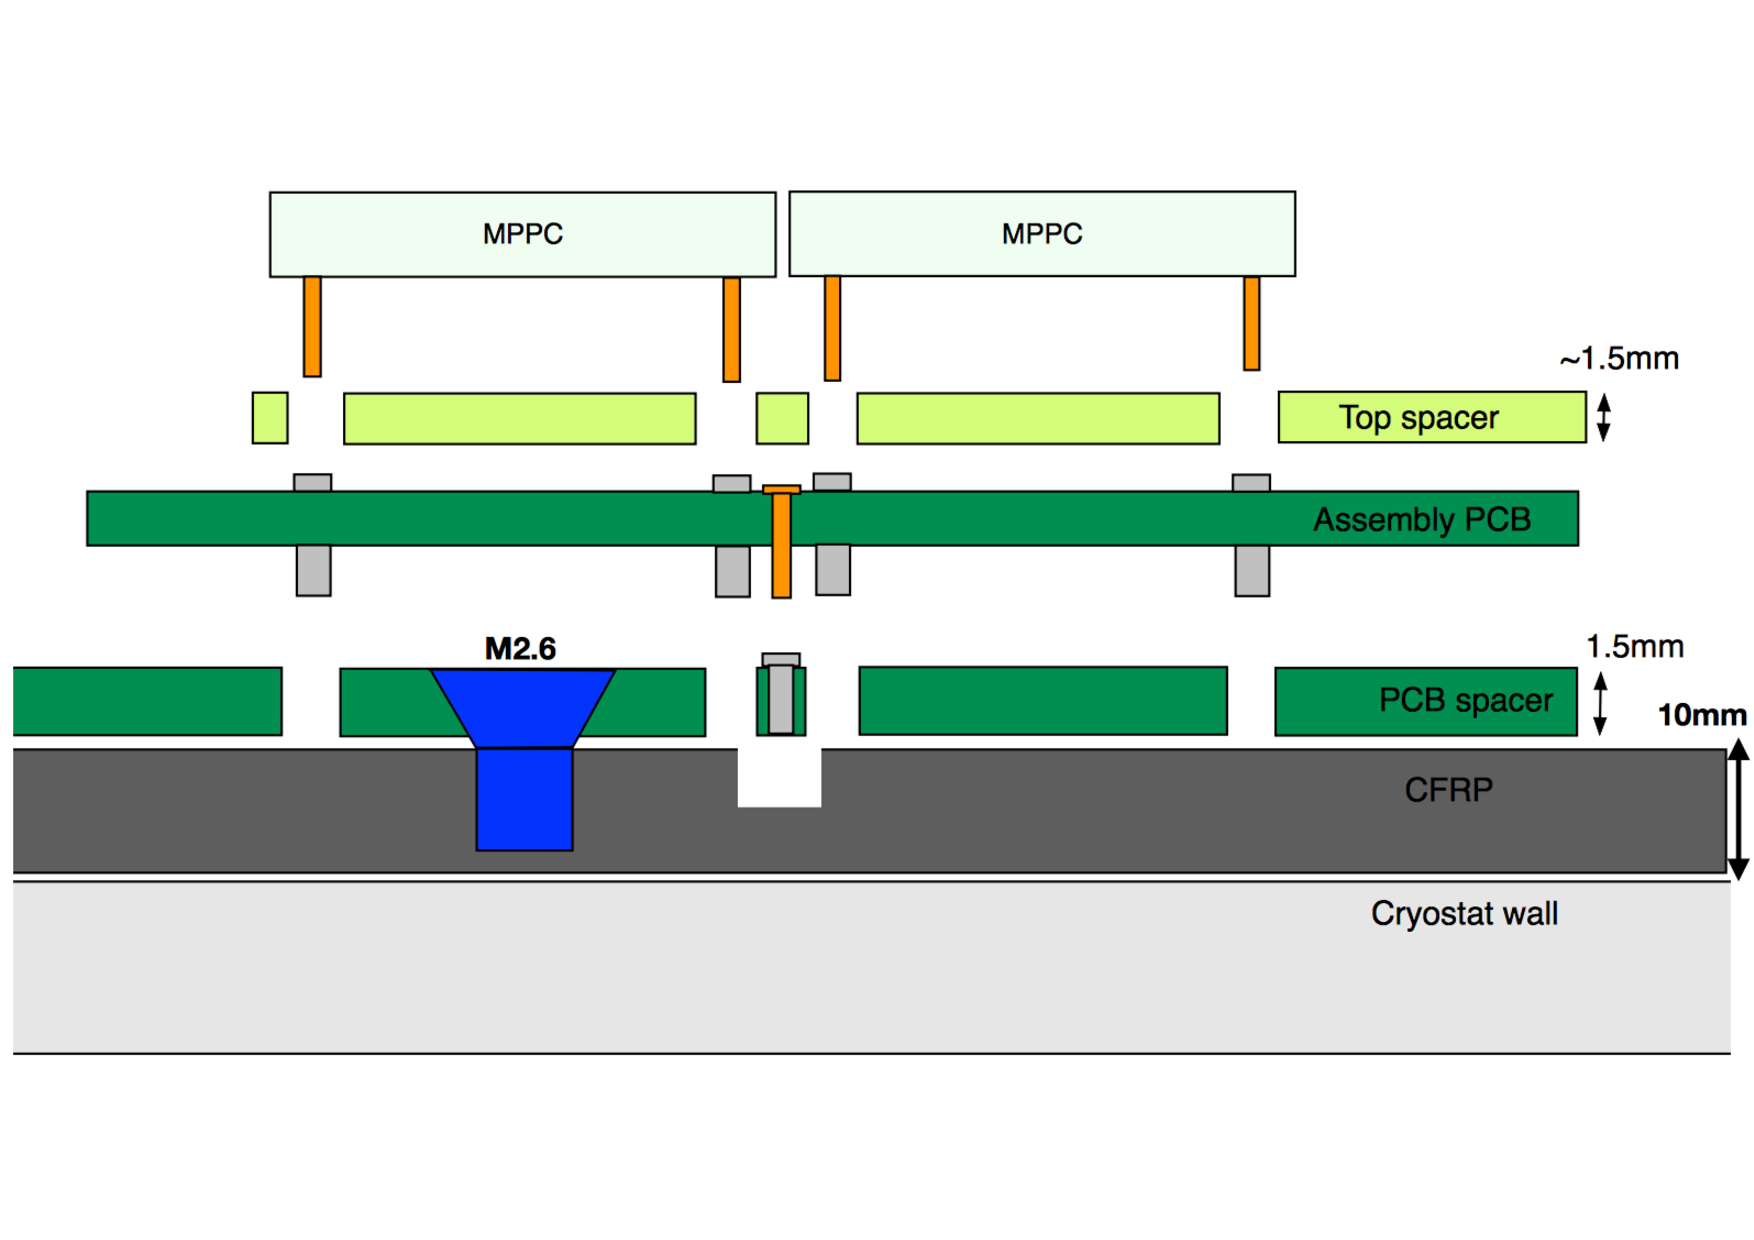
\includegraphics[width=4cm]{plots/MPPC_support.pdf}
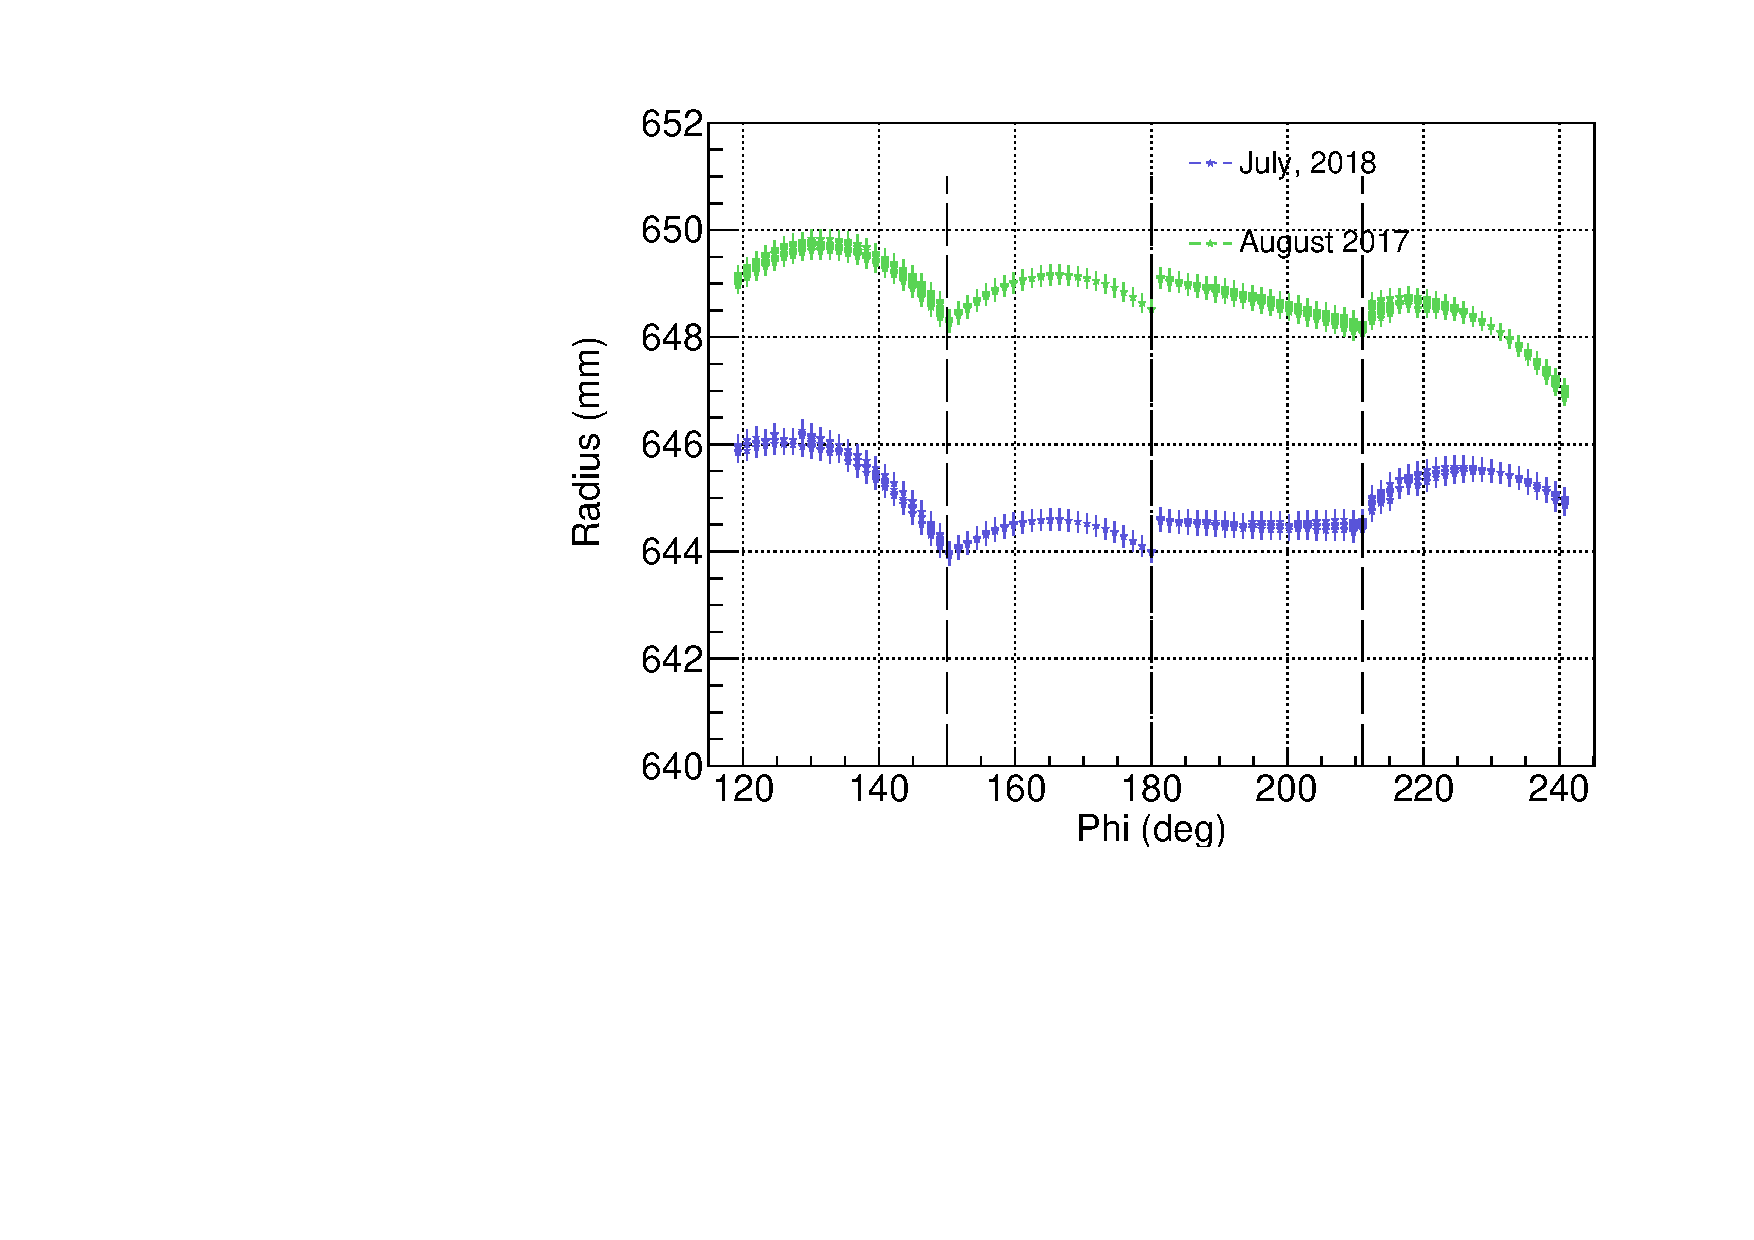
\includegraphics[width=4cm]{plots/2018/cRadius_1718}
\caption{ Radial coordinate of photodetectors with errors from 2017 and 2018
X-ray scans.  Black dashed lines indicate the edges of the CFRP plate.}
\label{fig:radiuscalculation} 
\end{center}
\end{figure}


\subsection { X-ray interaction rate -- 2017 vs 2018}  
The efficacy of spacer materials between MPPC, PCB strip and CFRP
plate is tested by examining the X-ray event rate as a function of
MPPC position. The rate is inversely proportional to the length of LXe
traversed by the X-ray before interaction.  It provides crucial
information about the state of spacer materials responsible for
preventing LXe leak between inner cryostat wall and the photosensitive
surface, which directly impacts photo detection and reconstruction
efficiencies, and energy response.  A constant rate of triggered
events is expected from all scanned MPPCs with some variation
attributed to electronic readouts that are nominally configured in an
identical way.  The event rates show a $\phi$ dependent variation
indicating some deformation in CFRP plates 1 and 2.  A drop in the
rates by a factor 1/e suggests the scale of deformation
$\approx\,\lambda_{\mathrm{Xe}}$.  The $\phi$ dependent variation is
observed in both Z and $\phi$ scans in the MPPCs illuminated with
X-rays and is not seen in the background process
(Figure~\ref{fig:ratesvszphi}).  The second scan in 2018 replicates
the previous years data at a lower rate due to reduced activity of the
source by two half-lives.  
\begin{figure}[]
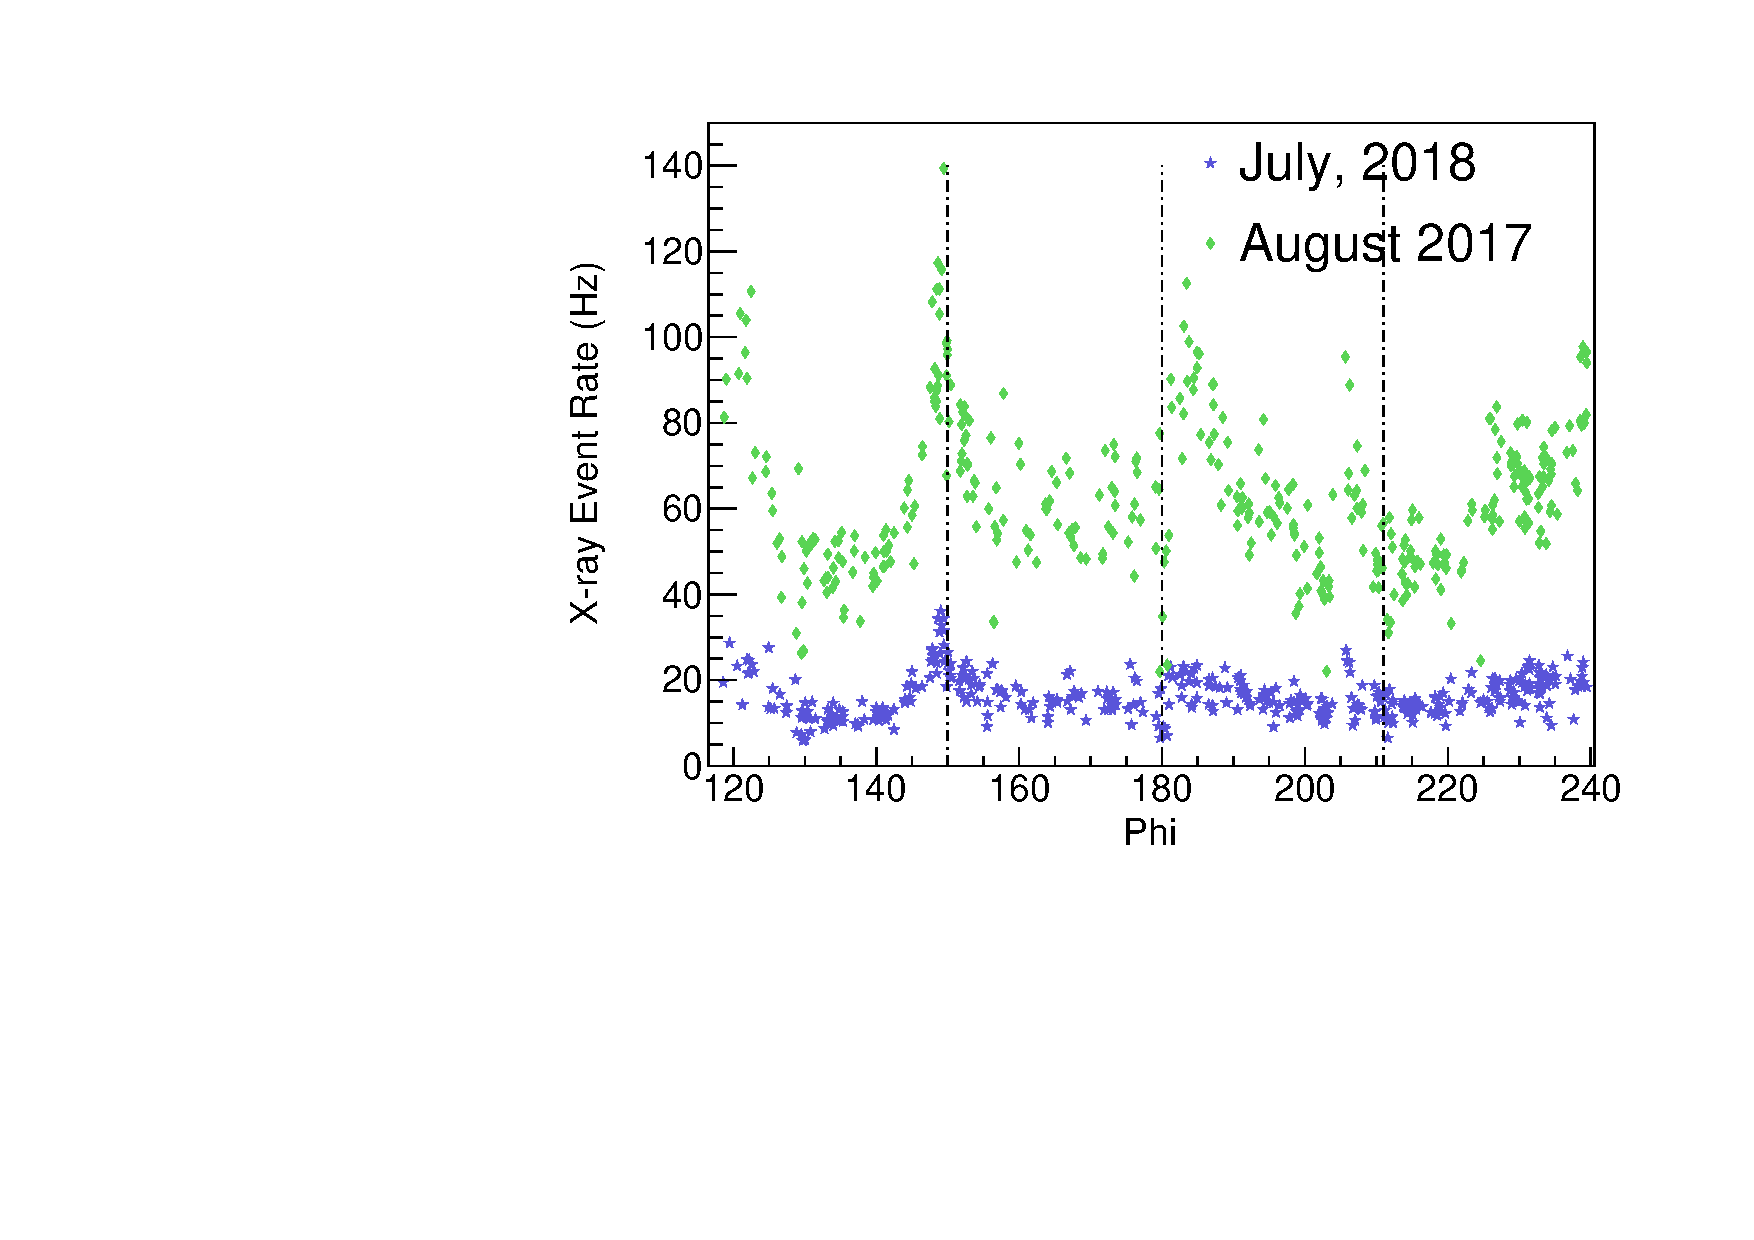
\includegraphics[width=4cm]{plots/2018/cEventRate_1718}
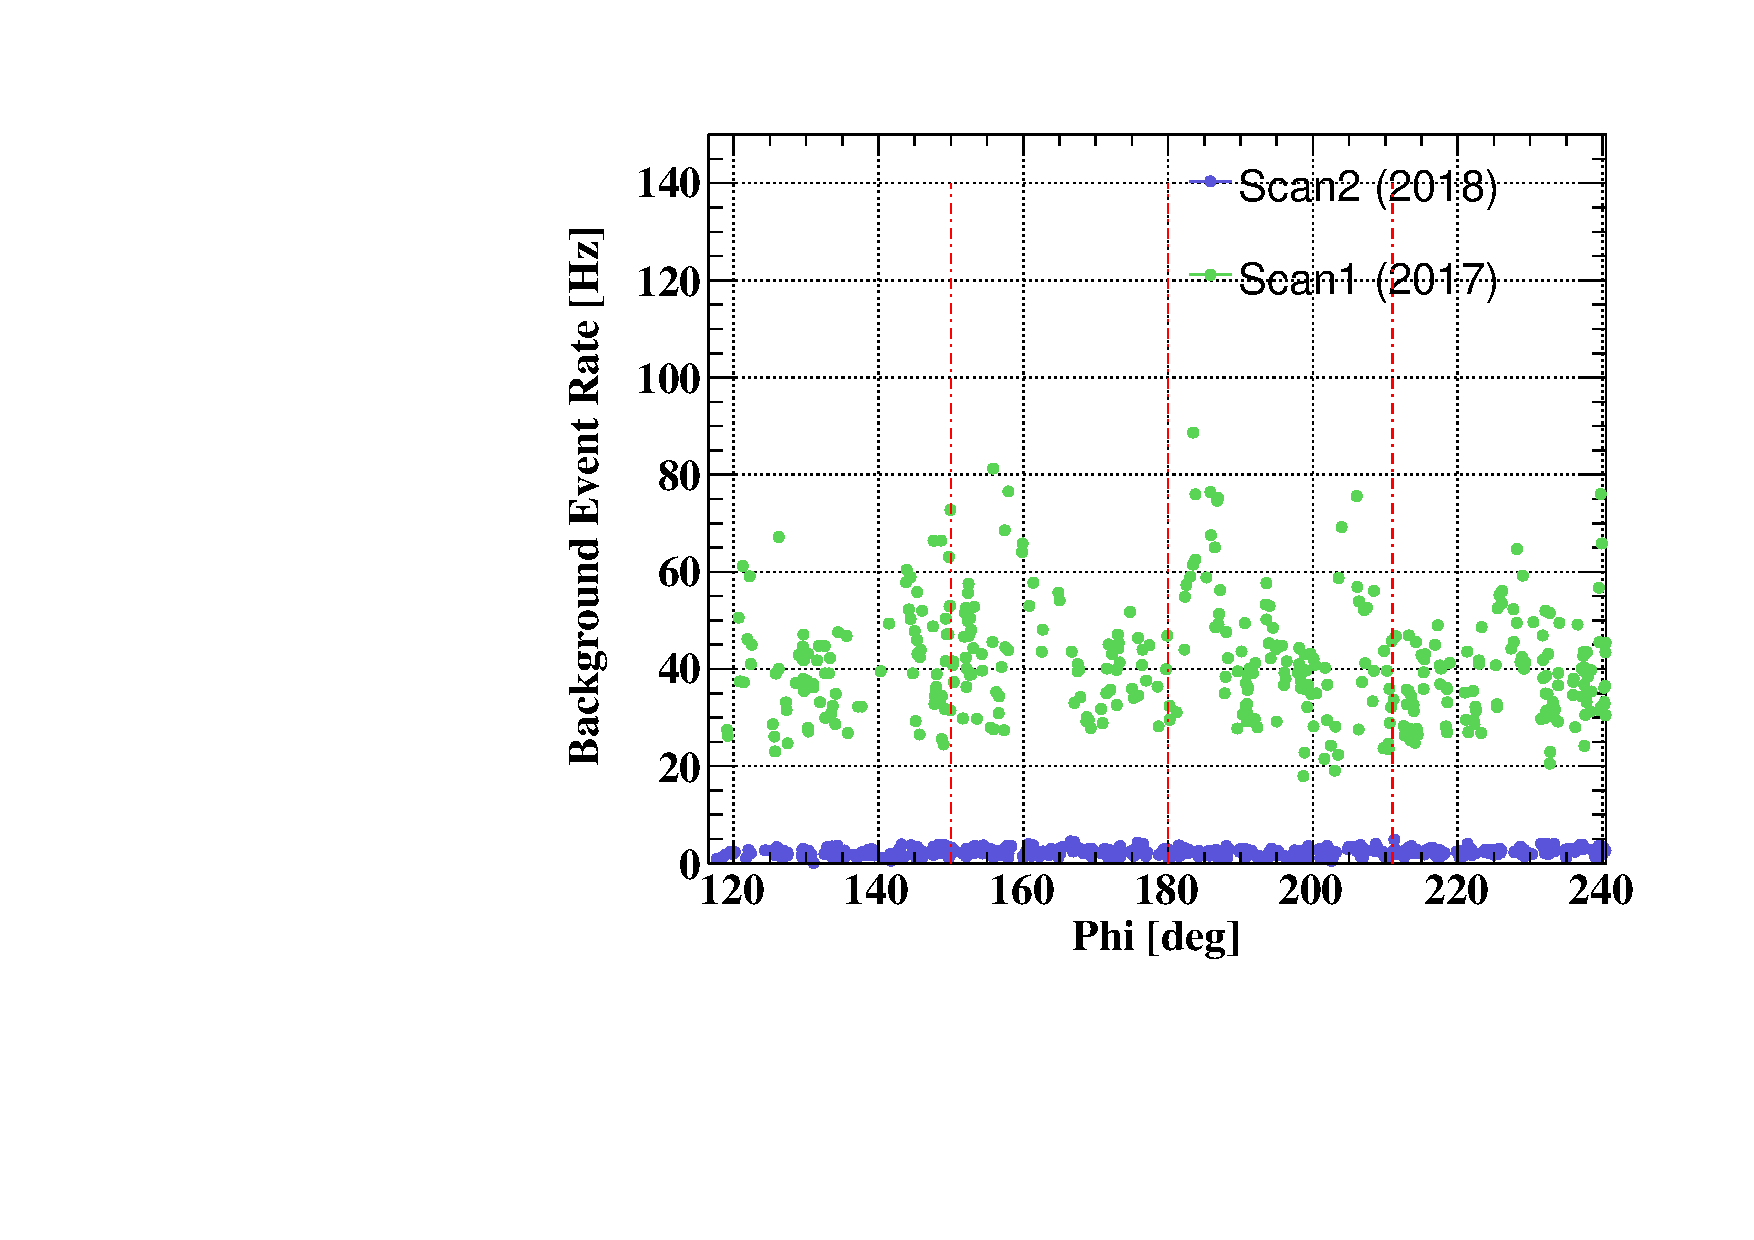
\includegraphics[width=4cm]{plots/2018/cBkgRate_1718} \caption{Signal
and background trigger rates observed in MPPC as a function of $\phi$.
Black lines indicate the edges of the CFRP plate.}
\label{fig:ratesvszphi} \end{figure}



\subsection{Charge Asymmetry} \label{sec:chargeasym}


An additional measurement of each photodetector's edge location was
determined by fitting charge asymmetries (Eqn. \ref{eqn:qasym}) between
adjacent photodetectors. This allows for a determination of
photodetector edges as defined by the midpoint between two detectors,
in which the X-ray induces charge measurements.

Event selection includes two classes of events; where the X-ray
induced charge is present in one of the channels, or shared by the two
adjacent channels.  The selection described in Sec.
\ref{sec:mppcposition} applied for single photodetector scan is used
with additional criteria to include events with X-ray interactions
between two photodetectors.  The requirement of minimal largest charge
in the single illuminated channel is reduced to 0.3~pC and the sum of
charges in the two illuminated channels is required to exceed 70\% of
total charge in the signal region.  Due to large variation in the gain
of individual photodetectors, the charge from each photodetector is
normarlized to avoid skewing the asymmetry distribution. The mean
charge is calculated for each photodetector in the central scanning
region and normalized before applying selection.

The charge asymmetry for a given photodetector $i$
is calculated per event are  calculated as  
\begin{equation} \label{eqn:qasym}
    A(Q)  = 
\frac{Q_{i}-Q_{i+1}}
     {Q_{i}+Q_{i+1}}, 
\end{equation}
where adjacent photodetector pairs ($i, i+1$) are chosen
along the direction of the coordinate scanned. The mean value
as a function of the coordinate is fitted to the 
following sigmoid function
\begin{equation}\label{eqn:asymfit}
f_{Asym}(z)=\;
C\,\left[\,Erfc(a(z-z_{0}))-1\,\right],
\end{equation} 
where $z_0$ is the offset in Z, and $C$ and $a$ are 
the scaling parameters of the function.

The center of the asymmetry distribution, $A(Q)=0$ in fig.
\ref{fig:asymplot}, consistutes the physical edge of the
photodetector.  Using both edges, the photodectector position and its
size is independently calculated, in each Z and \phis coordinate.  A
comparison between calculated photodetector position using X-ray event
rates and charge asymmetry (fig. \ref{fig:asymvsfit}) shows the two
measurements to be consistent.  The photodetector size calculated with
asymmetry (fig. \ref{fig:mppcsize}) is also in good agreement with the
average spacing of the photodetectors previously calculated (table
\ref{tab:avgspacing}).  Due to trigger configuration and the
particular scanning region used in the X-ray survey, photodetectors on
the boundary of trigger region are excluded from the calculaton,
limiting this measurement to 15\% of the scanned photodetectors.


\begin{figure}
\centering
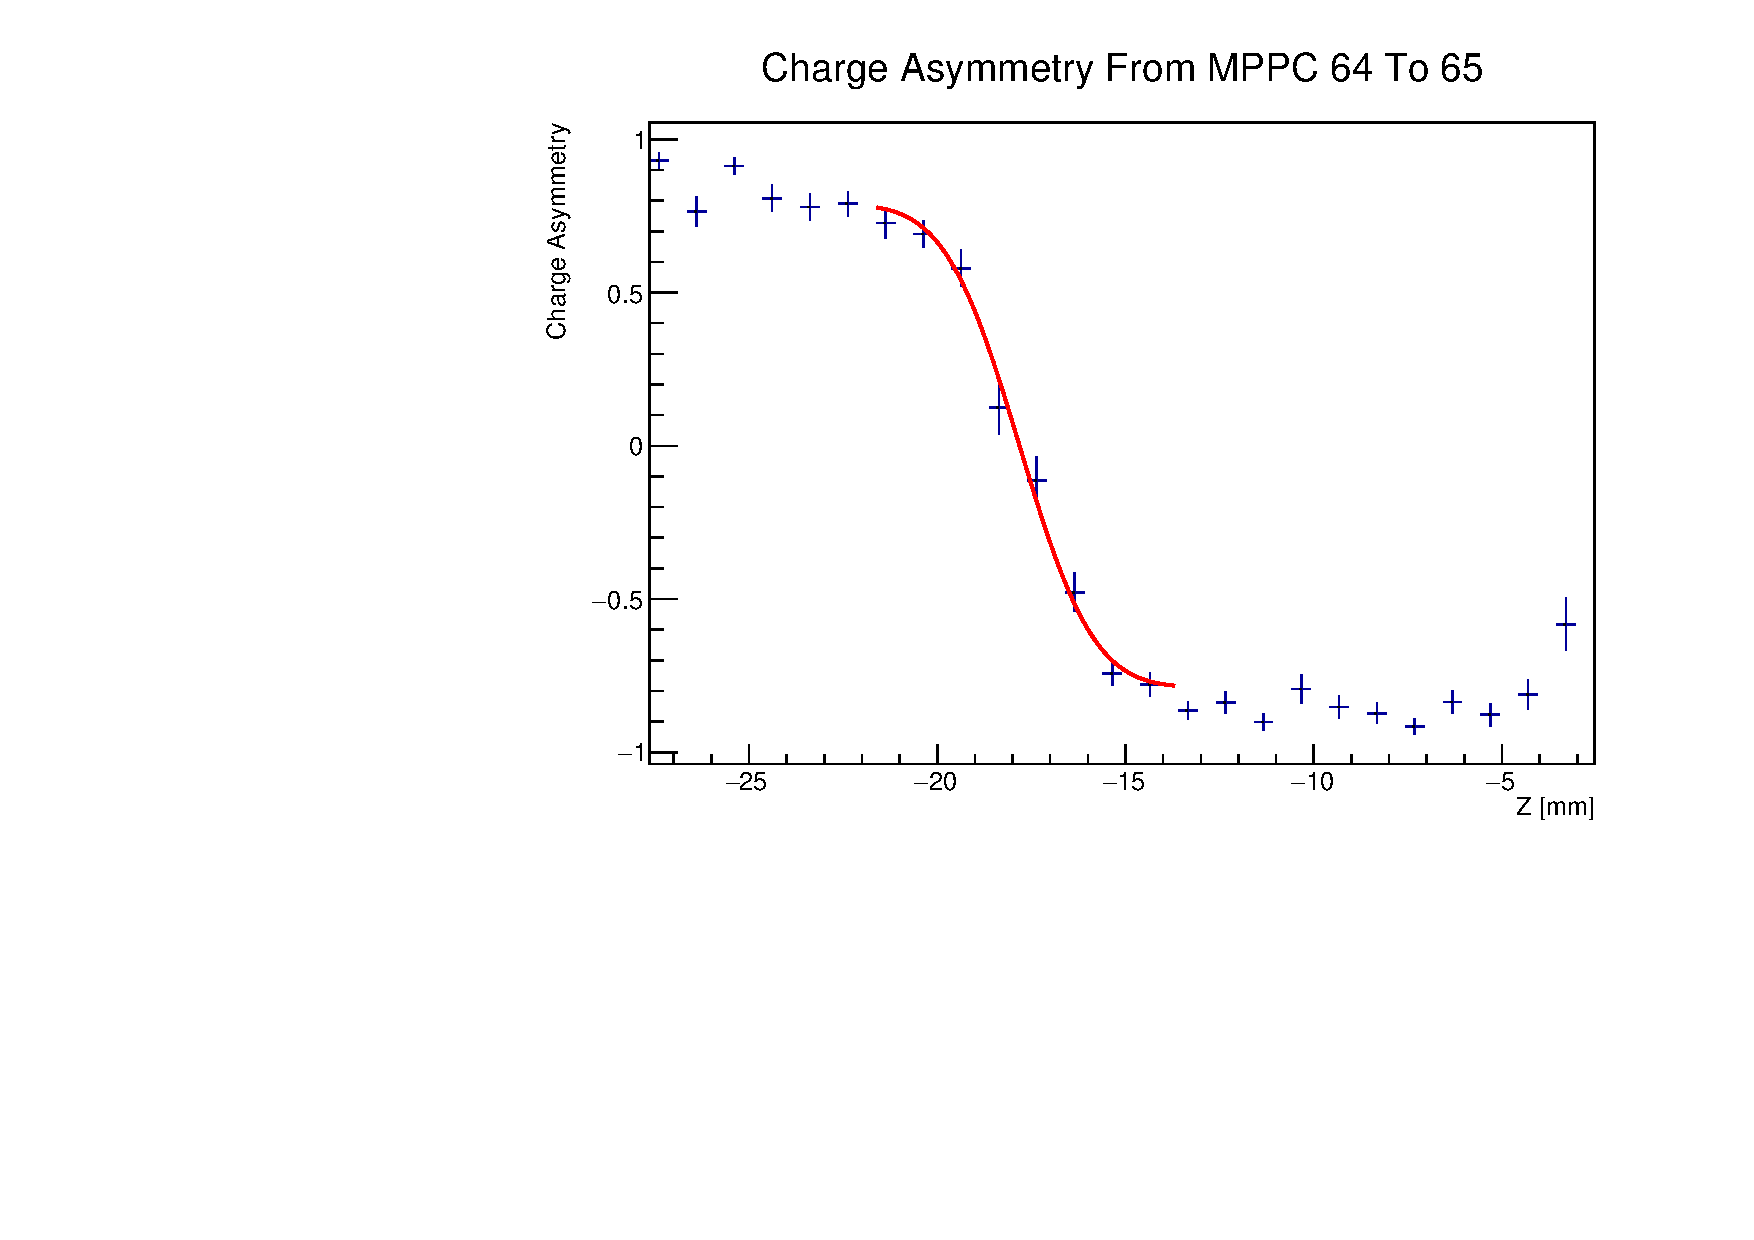
\includegraphics[width=4cm]{graphics/asym6465.pdf}
\caption{Mean charge asymmetry calculated as a function of z between 
two photodetectors.}
\label{fig:asymplot} 
\end{figure}

\begin{figure}
\centering
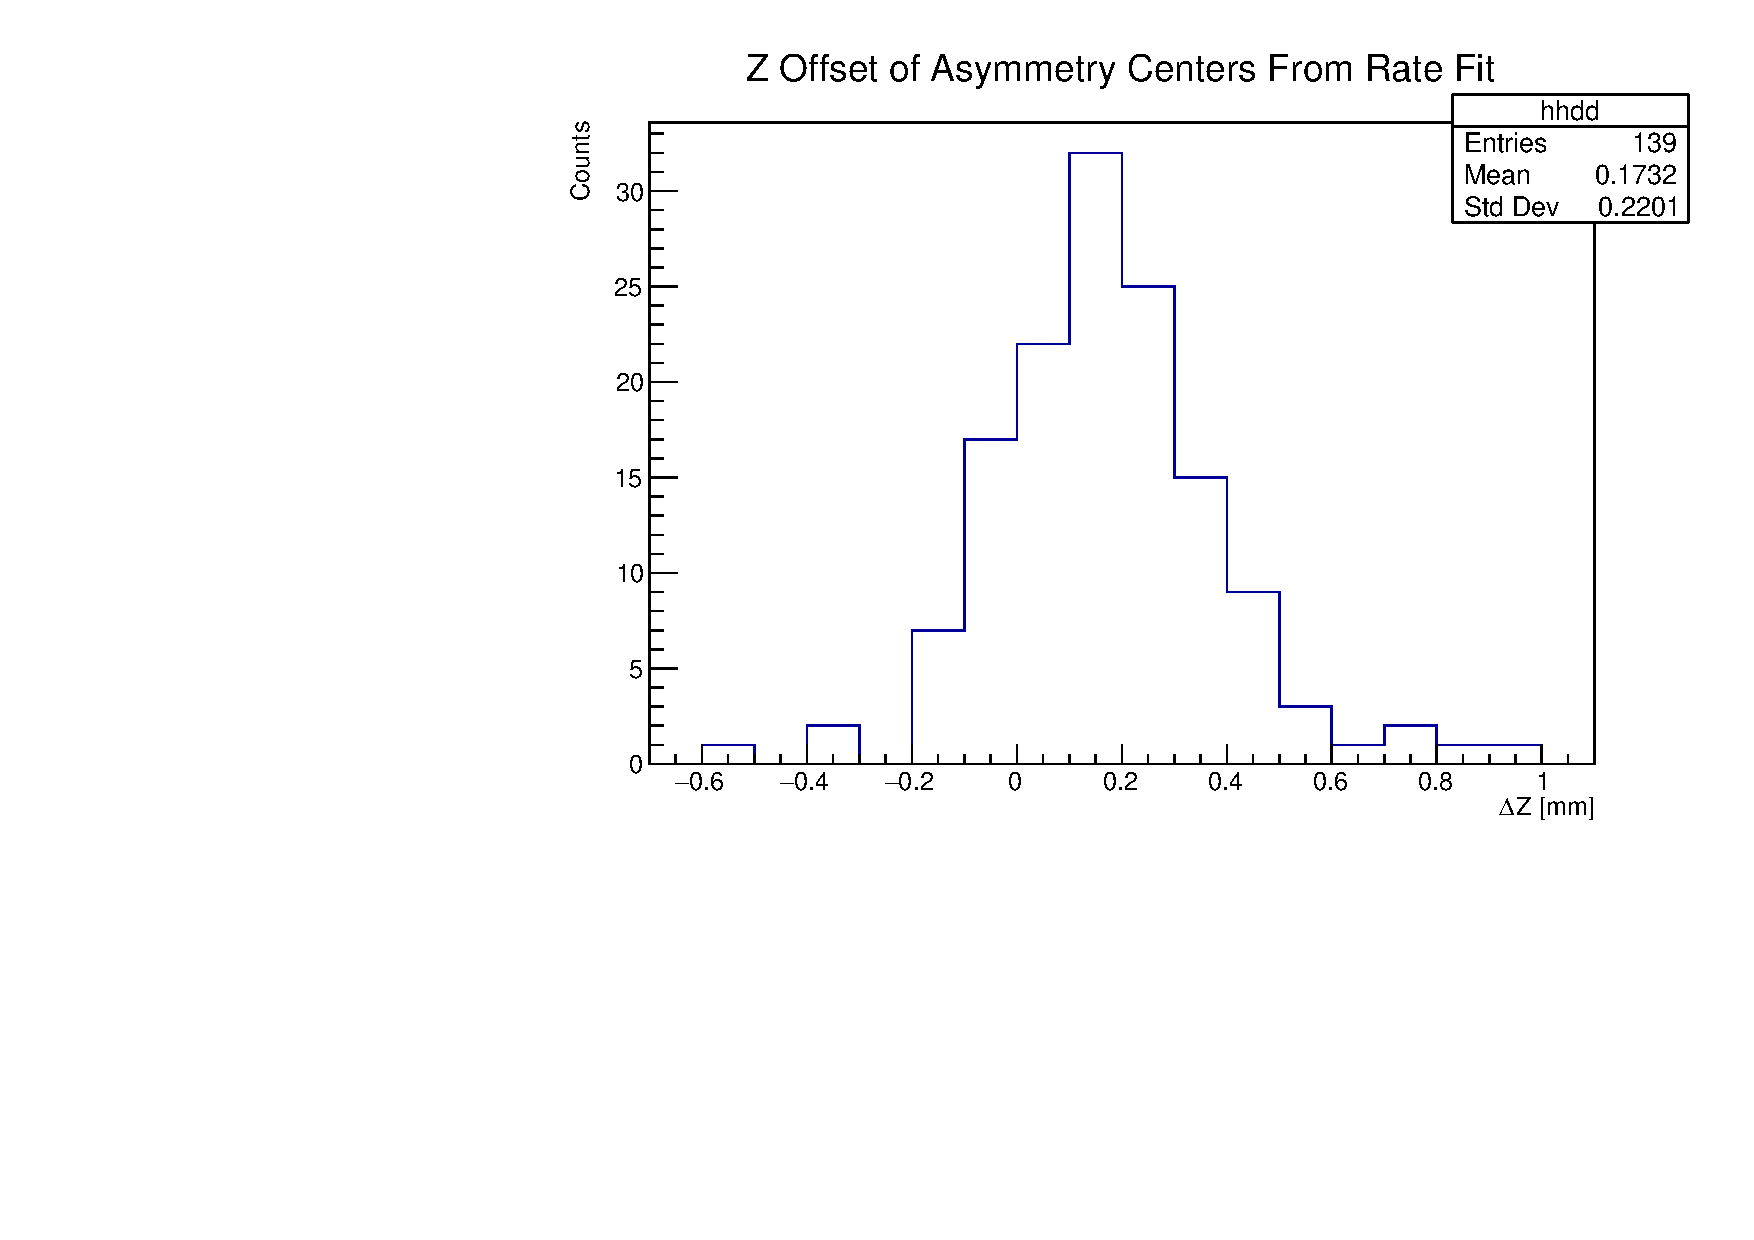
\includegraphics[width=4cm]{asymmetryplots/asymzoffset.pdf}
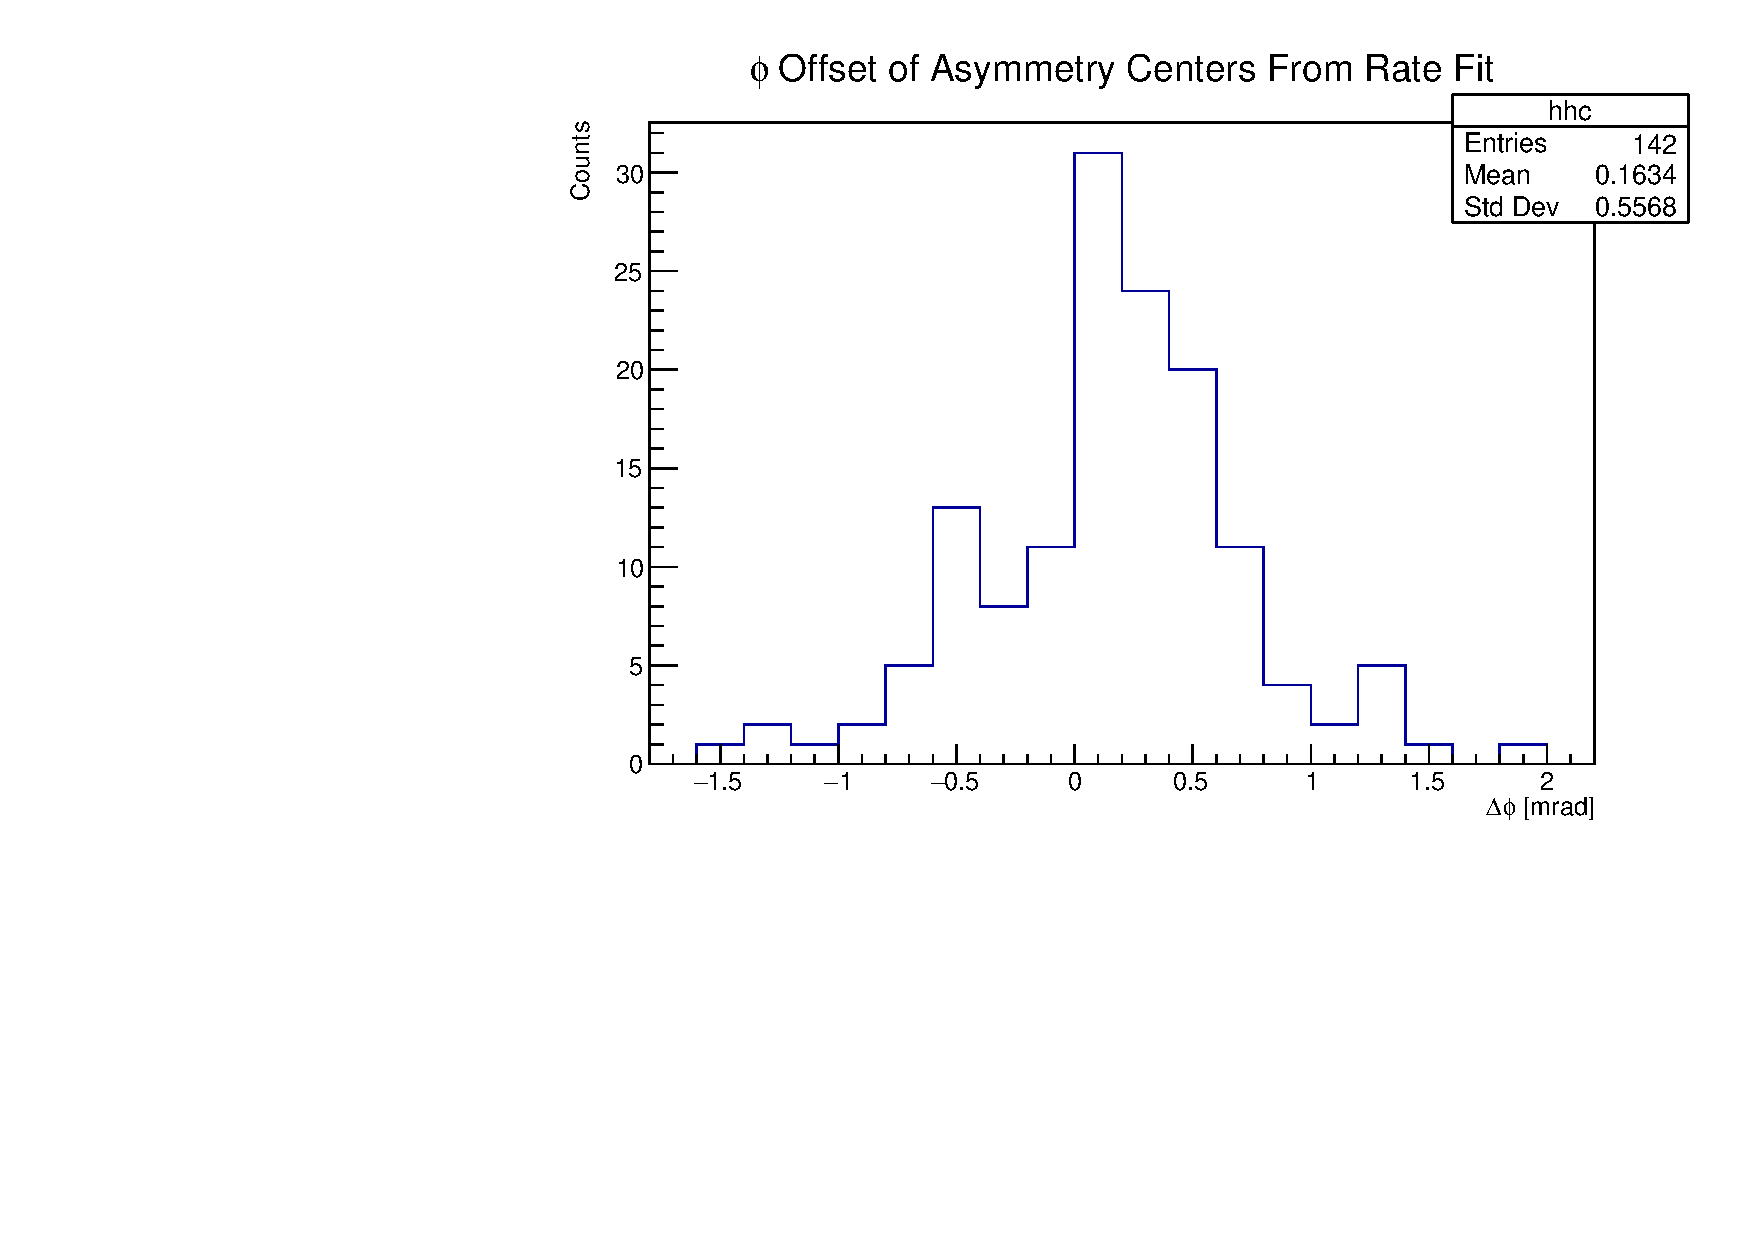
\includegraphics[width=4cm]{asymmetryplots/asymphioffset.pdf}
\caption{Comparison between photodetector position calculated from
charge asymmetry and X-ray event rates.}
\label{fig:asymvsfit} 
\end{figure}



\begin{figure}
\centering
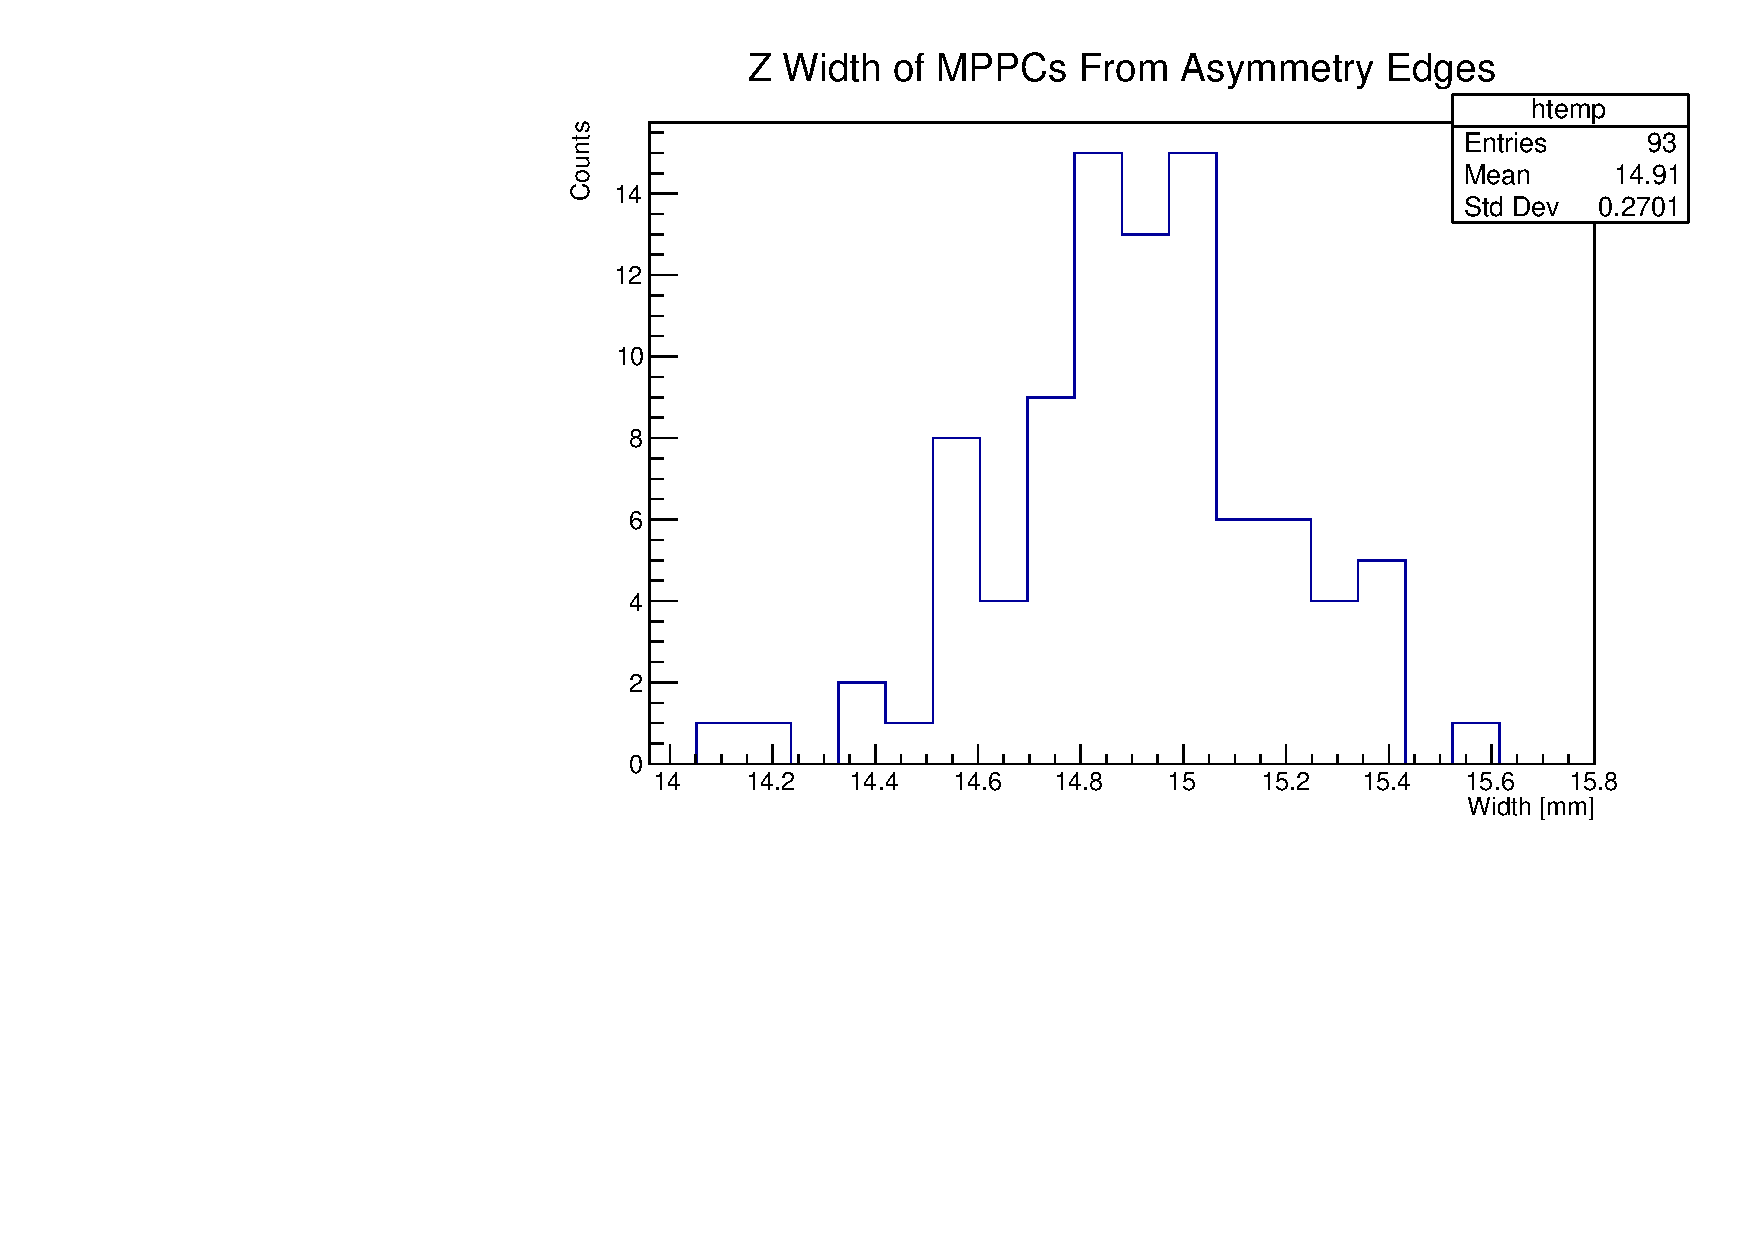
\includegraphics[width=4cm]{asymmetryplots/asymzwid.pdf}
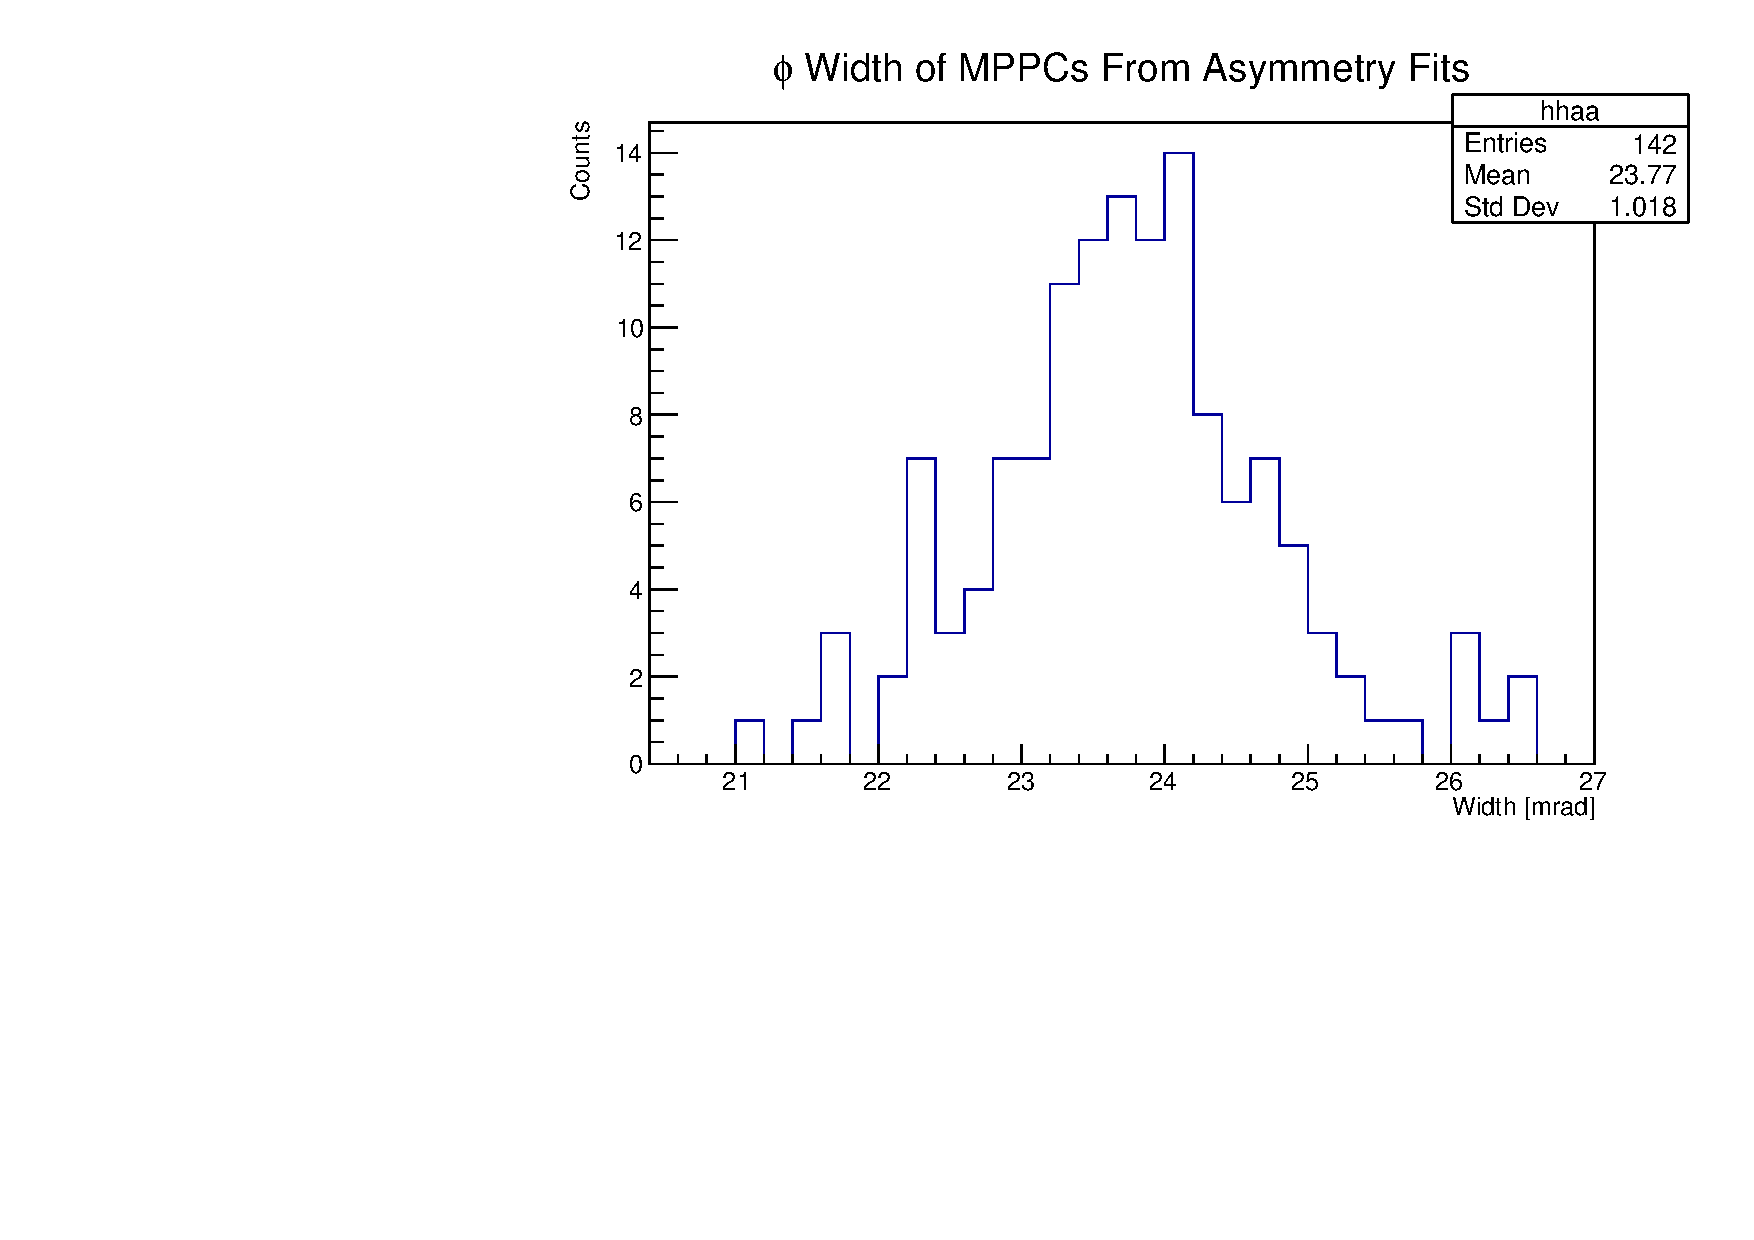
\includegraphics[width=4cm]{asymmetryplots/asymphiwid.pdf}
\caption{Photodetector size in Z and phi measured using the edge of the
photodetector calculated with charge asymmetry.}
\label{fig:mppcsize} 
\end{figure}



%With these additional measurements, it is possible to produce a
%comparison to our prior findings on the photodetector spacing. For
%this purpose, we calculate all the possible offsets of detectors edges
%(per asymmetry fits) from their previously fitted central locations. 

%%%%%%%\begin{table}[H]
%%%%%%%    \centering
%%%%%%%    \begin{tabular}{c||c|c}
%%%%%%%        \bf Upper Edge & \bf \boldmath$\mu$ [mm] & \bf \boldmath$\sigma_{RMS}$ [mm] \\
%%%%%%%         \hline
%%%%%%%        Even, 1 of 4 & 7.954 & 0.500 \\
%%%%%%%        Even, 3 of 4 & 7.824 & 0.409 \\
%%%%%%%        Even, 1 of 2 & 7.82 & 0.438  \\
%%%%%%%        Odd, 2 of 4 & 7.713 & 0.396  \\
%%%%%%%        \hline
%%%%%%%        All Even & 7.862 & 0.451 \\
%%%%%%%        All Odd & 7.713 & 0.396
%%%%%%%    \end{tabular}
%%%%%%%    \caption{Measured Z Offsets of Upper Edges From Fit Centers}
%%%%%%%    \label{tab:upperedgeasymz}
%%%%%%%\end{table}
%%%%%%%
%%%%%%%\begin{table}[H]
%%%%%%%    \centering
%%%%%%%    \begin{tabular}{c||c|c}
%%%%%%%         \bf Lower Edge & \bf \boldmath$\mu$ [mm] & \bf \boldmath$\sigma_{RMS}$ [mm] \\
%%%%%%%         \hline
%%%%%%%         Odd, 2 of 4 & 7.363 & 0.385 \\
%%%%%%%         Odd, 4 of 4 & 7.771 & 0.413 \\
%%%%%%%         Odd, 2 of 2 & 7.816 & 0.410 \\
%%%%%%%         Even, 3 of 4 & 7.154 & 0.436 \\
%%%%%%%         \hline 
%%%%%%%         All Even & 7.154 & 0.436 \\
%%%%%%%         All Odd & 7.669 & 0.448
%%%%%%%    \end{tabular}
%%%%%%%    \caption{Measured Z Offsets of Lower Edges From Fit Centers}
%%%%%%%    \label{tab:loweredgeasymz}
%%%%%%%\end{table}
%%%%%%%
%%%%%%%\begin{table}[H]
%%%%%%%    \centering
%%%%%%%    \begin{tabular}{c||c|c}
%%%%%%%        \bf Upper Edge & \bf \boldmath$\mu$ [mrad] & \bf \boldmath$\sigma_{RMS}$ [mrad] \\
%%%%%%%         \hline
%%%%%%%        Even, 1 of 4 & 12.05 & 1.023 \\
%%%%%%%        Even, 3 of 4 & 12.56 & 0.7336 \\
%%%%%%%        Even, 1 of 2 & 12.28 & 0.357  \\
%%%%%%%        Odd, 2 of 4 & 12.23 & 1.125  \\
%%%%%%%        \hline
%%%%%%%        All Even & 12.32 & 0.884 \\
%%%%%%%        All Odd & 12.23 & 1.125
%%%%%%%    \end{tabular}
%%%%%%%    \caption{Measured $\phi$ Offsets of Upper Edges From Fit Centers}
%%%%%%%    \label{tab:upperedgeasymphi}
%%%%%%%\end{table}
%%%%%%%
%%%%%%%\begin{table}[H]
%%%%%%%    \centering
%%%%%%%    \begin{tabular}{c||c|c}
%%%%%%%         \bf Lower Edge & \bf \boldmath$\mu$ [mrad] & \bf \boldmath$\sigma_{RMS}$ [mrad]\\
%%%%%%%         \hline
%%%%%%%         Odd, 2 of 4 & 11.87 & 0.715 \\
%%%%%%%         Odd, 4 of 4 & 11.99 & 0.629 \\
%%%%%%%         Odd, 2 of 2 & 11.83 & 0.340 \\
%%%%%%%         Even, 3 of 4 & 11.42 & 0.717 \\
%%%%%%%         \hline
%%%%%%%         All Even & 11.42 & 0.717 \\
%%%%%%%         All Odd & 11.93 & 0.654
%%%%%%%    \end{tabular}
%%%%%%%    \caption{Measured $\phi$ Offsets of Lower Edges From Fit Centers}
%%%%%%%    \label{tab:loweredgeasymphi}
%%%%%%%\end{table}
%%%%%%%
%%%%%%%Included above is a separation based upon location of each measurement
%%%%%%%within the trigger region of a scan, and is listed as an index from 1
%%%%%%%to either 2 or 4, depending upon the number of detectors the beam
%%%%%%%traversed within a scan.



%%\subsection{Charge Asymmetry}
%%\noindent Definition \\
%%Selection of events \\
%%Charge (sharing) fraction between adjacent mppc \\
%%Gain equalization and fitting  \\
%%Comparison to earlier calculations of position and spacing. \\


\subsection{Quantum Efficiency$\times$Gain}
An uniform source of light provided by the collimated X-ray beam is
used to measure relative gain of the photodetectors.  The mean charge
response, proportional to the gain and quantum efficiency, is measured
with a good spatial precision in the X-ray survey.  Assuming the
quantum efficiencies are identical, the mean charge response is
analyzed to determine the stability and uniformity of photodetector
gain over the scanned region of the calorimeter.  It must be noted
that the charge measurement contains smaller but inseparable
contributions from after-pulse and cross-talk between neighboring
photodetectors, which are independent from the photodetector gain.
Additionally, only relative measurement of gain is possible as the
absolute photon yield in the X-ray interaction relies on other factors
such as presence of impurities in the liquid Xenon which were not
precisely known. 


The photodetectors are developed according to the experimental
requirements with large photosensitive area 12 $\times$ 12 mm$^2$,
comprised of four  smaller pixels 6 $\times$ 6 mm$^2$ connected in
series.  The photodetectors are placed in a ceramic case (15 mm) and
mounted on a PCB strip, each containing 22 photodetectors.  Two
identically produced strips aligned along $\hat{z}$ direction, and
rotated by 180\degree with respect to each other to allow for
electronics readout at each end, make up a single row (fig 
\ref{fig:mppc}).
The mean charge  is calculated over the 12 mm region centered at the
fitted photodetector location from previous analysis.  Due to long
tail in the charge distribution an iterative gaussian fit is used,
initially over the entire range and then restricted to the two sigma
region of the first fit.  The mean charge varies overall between the
scanned photodetectors by 50\%, and correlates reliably with the
production batch of the photodetectors (fig \ref{fig:mppccharge}). 

\begin{figure}
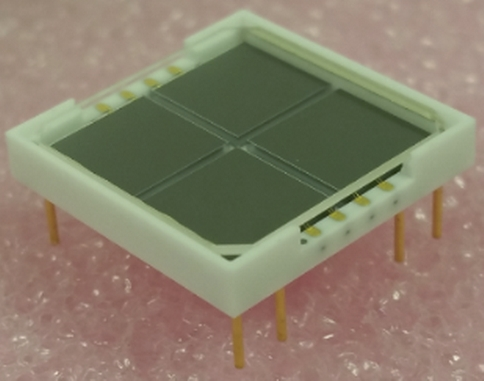
\includegraphics[width=3cm]{plots/single_mppc.jpg}
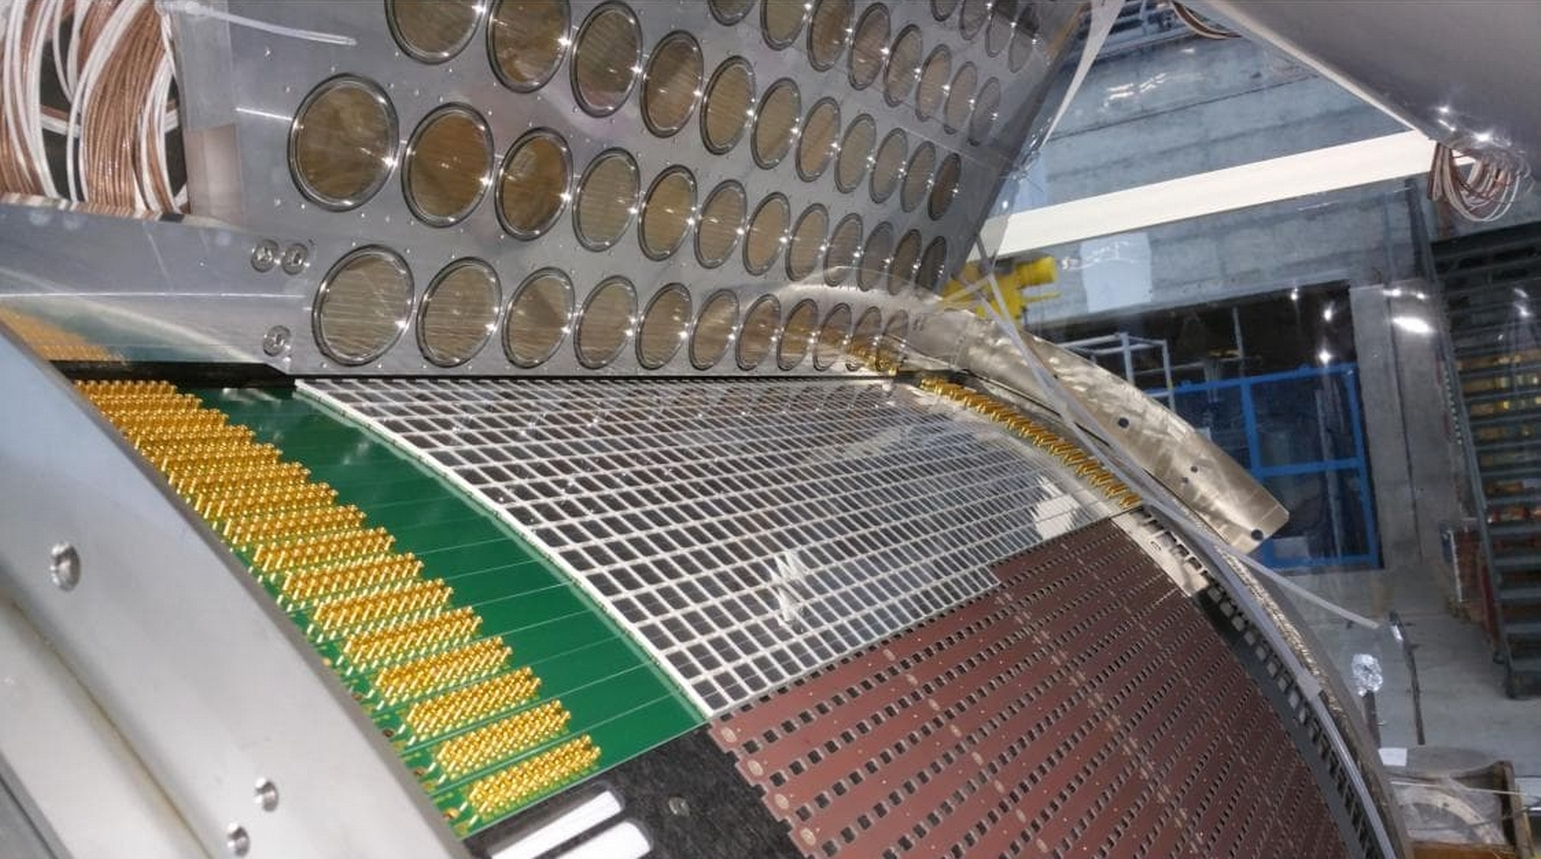
\includegraphics[width=5cm]{plots/CFRP_spacer_MPPC.jpg}
\caption{Single MPPC and installed MPPCs in the LXe calorimeter.}
\label{fig:mppc} 
\end{figure}

\begin{figure}
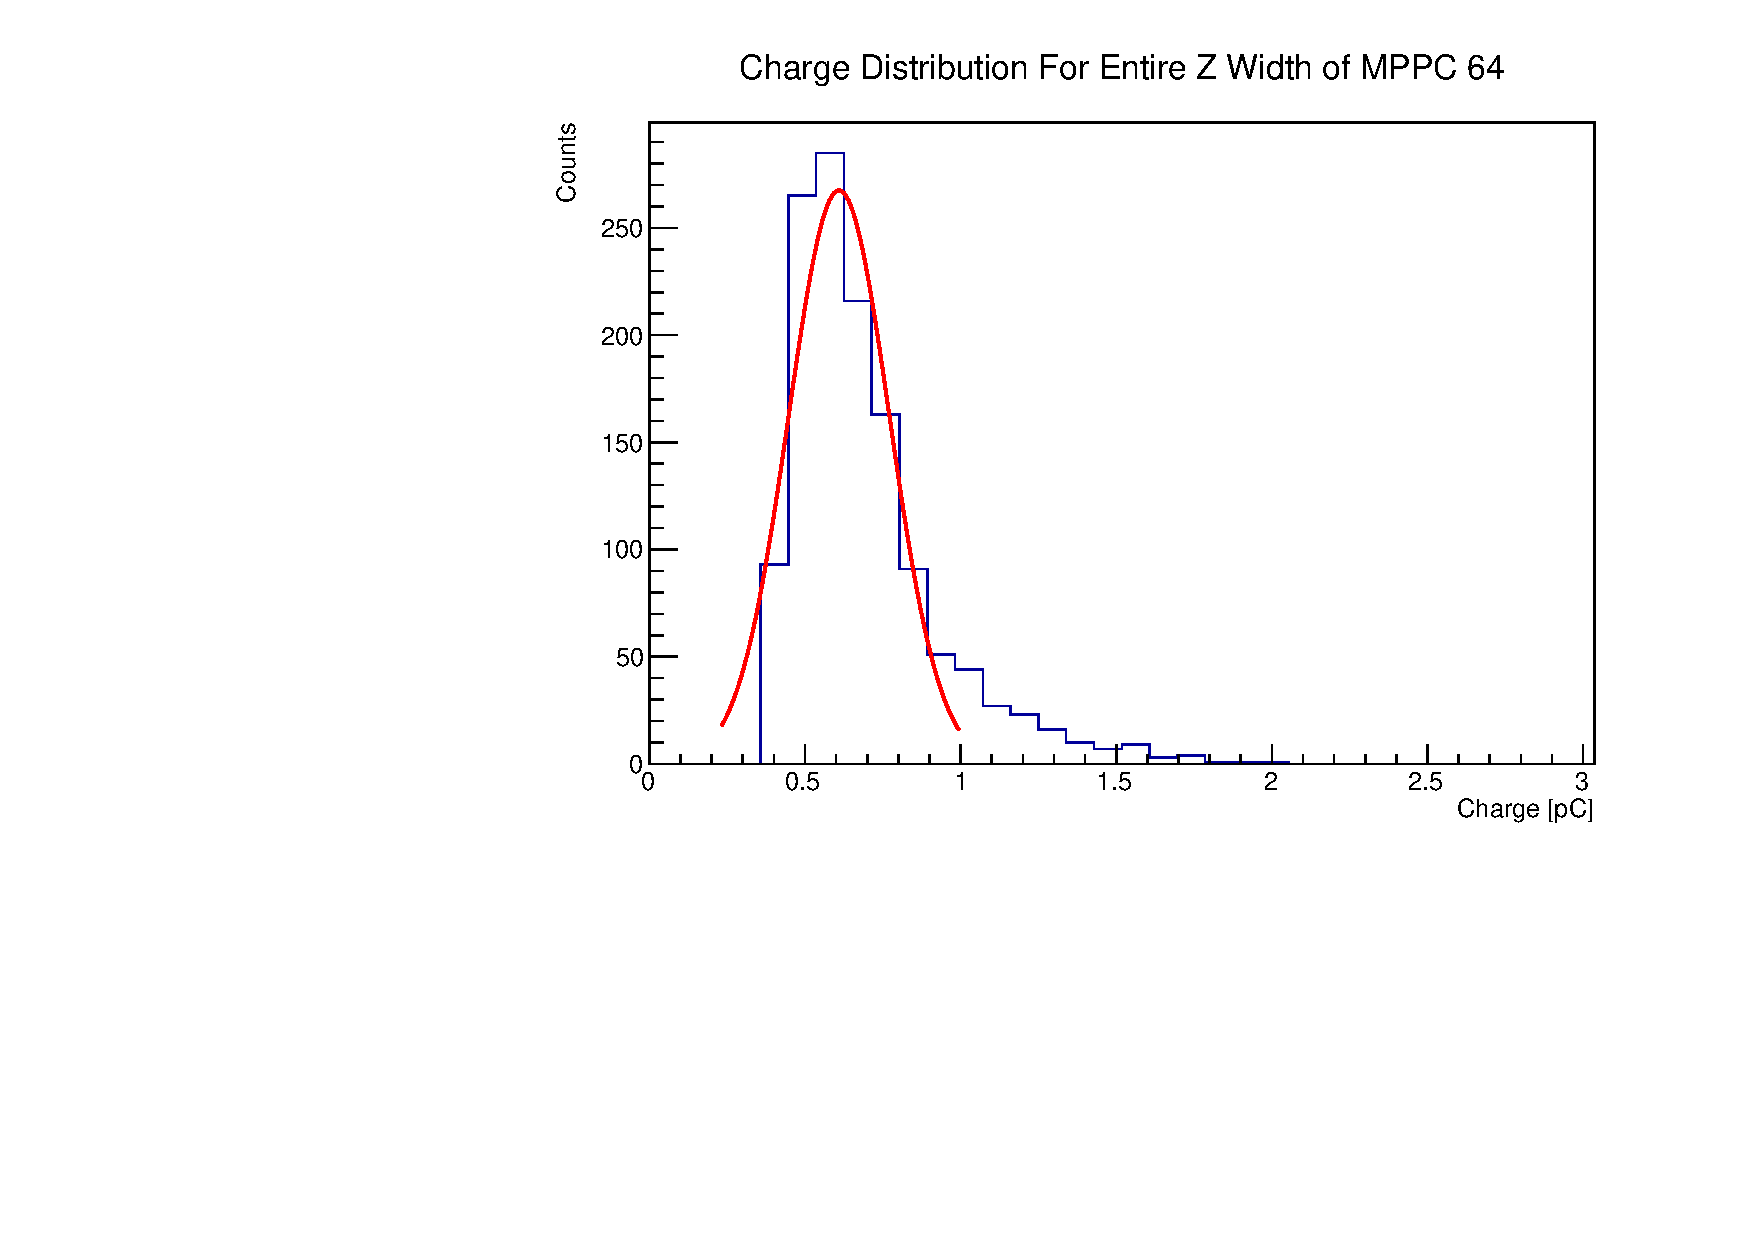
\includegraphics[width=4cm]{plots/2018/qgaindist64.pdf}
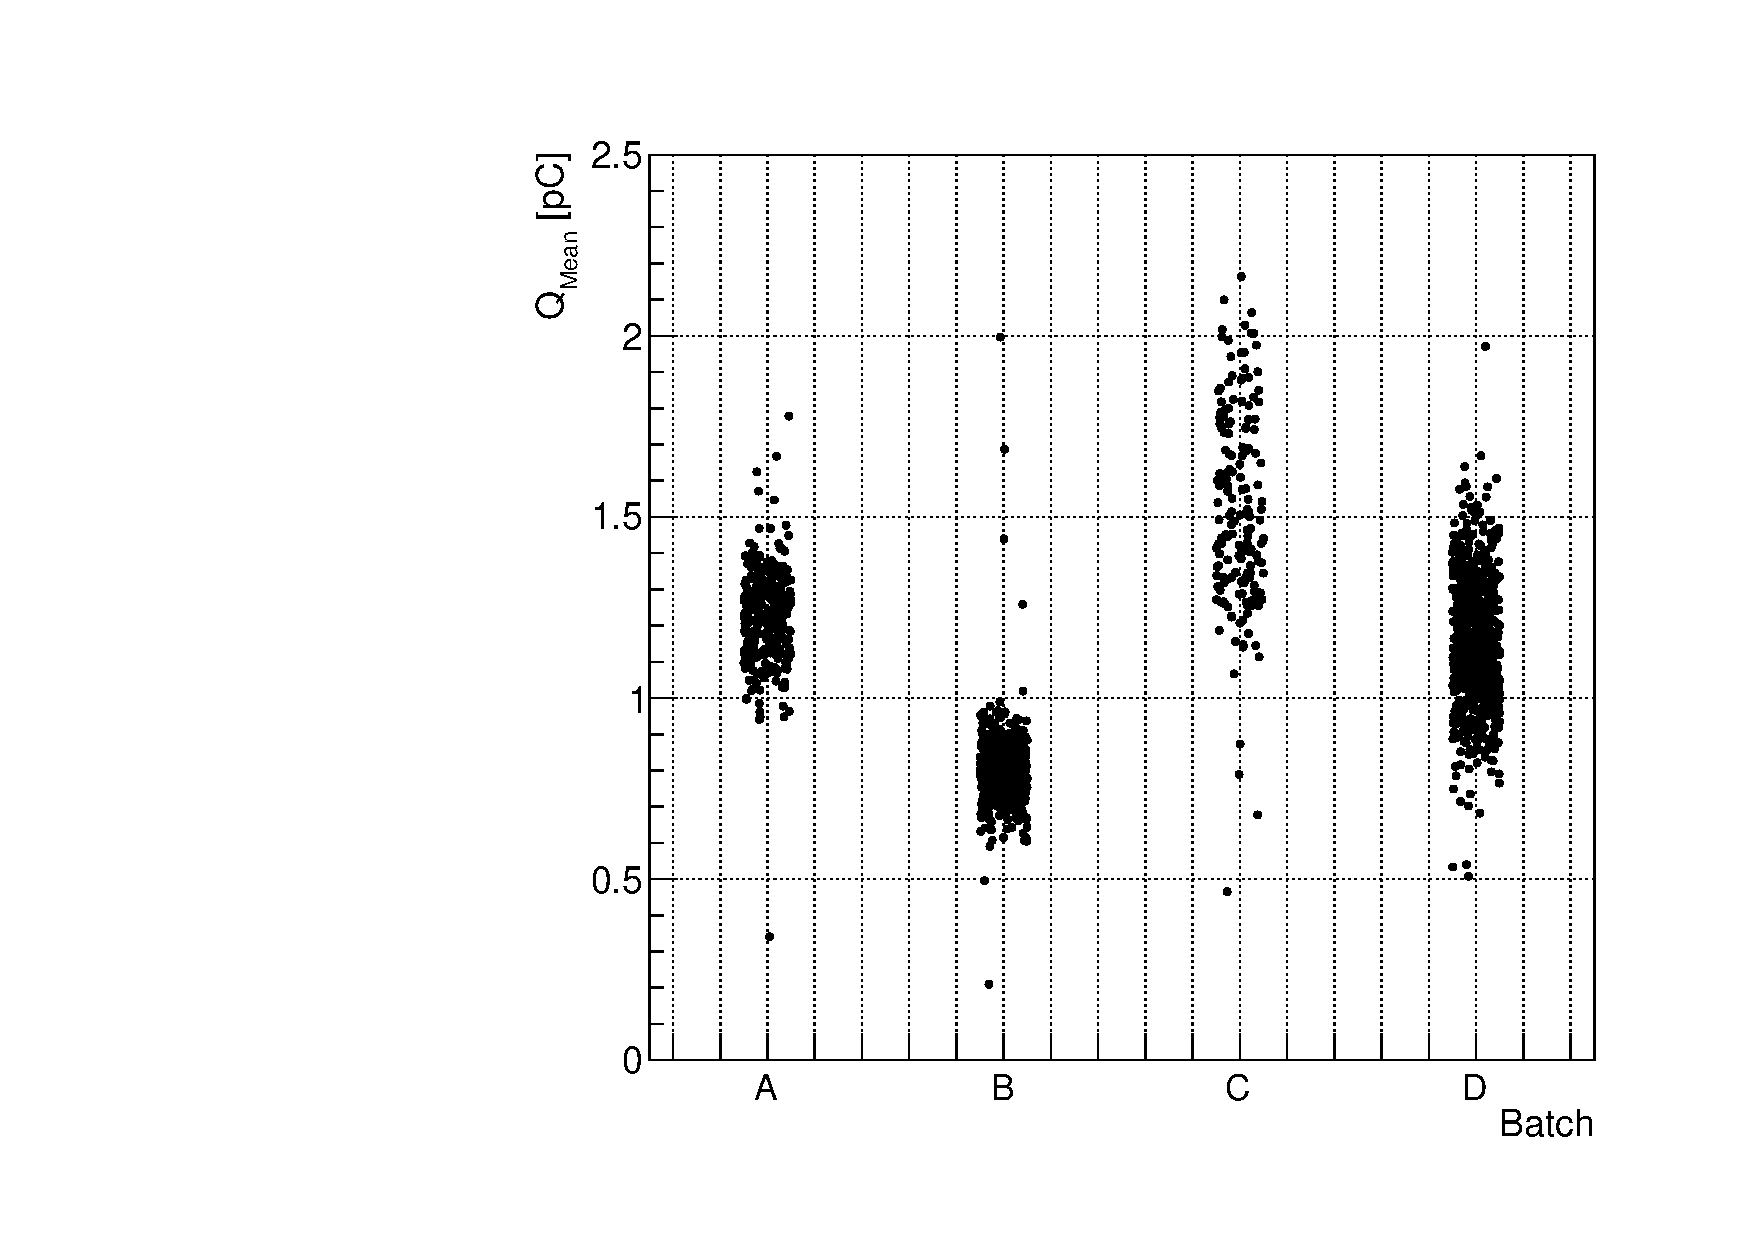
\includegraphics[width=4cm]{plots/2018/qmean_vs_batch.pdf}
\caption{Charge measured in a single MPPC with gaussian fit (left).
Mean charge measured measured in the batch (right). }
\label{fig:mppccharge} 
\end{figure}

The fine scanning resolution (scanning step 1 mm in z and \phis, and
X-ray beam size  $\sim$ 1 mm), is used to determine variation in
charge response of the component pixels of the photodetector.  The
position dependent variation in mean charge seen in figure
\ref{fig:xrayevents} demonstrates the difference in the response of
half photodetector  (two of four pixels) illuminated at every
position.  A visible decrease at the center of the photodetector is
caused by the central gap between the two rows of pixels.  Mean charge
in each half of the photodetector is independently calculated about
the center position determined in the previous analysis.  We find that
the mean charge varies between the two halves seperated by their Z
coordinate by 10\% and equal in the two halves separated by \phis.  Due
to the relative rotation the PCB strips per row about the center, the
mean charge of each half of the photodetector is also swapped
accordingly (fig \ref{fig:pixelcharge}). 
This disparity in charge response
is found to be independent of the production batch of the 
photodetector, observed at consistent level across all
batch groups.

An analysis of gain equalized charge measurements
was performed to assess its impact on the calculated 
photodetector position. There was no significant change
in the photodetector position with the resolution
degrading marginally by 0.05 mm. 

\begin{figure}
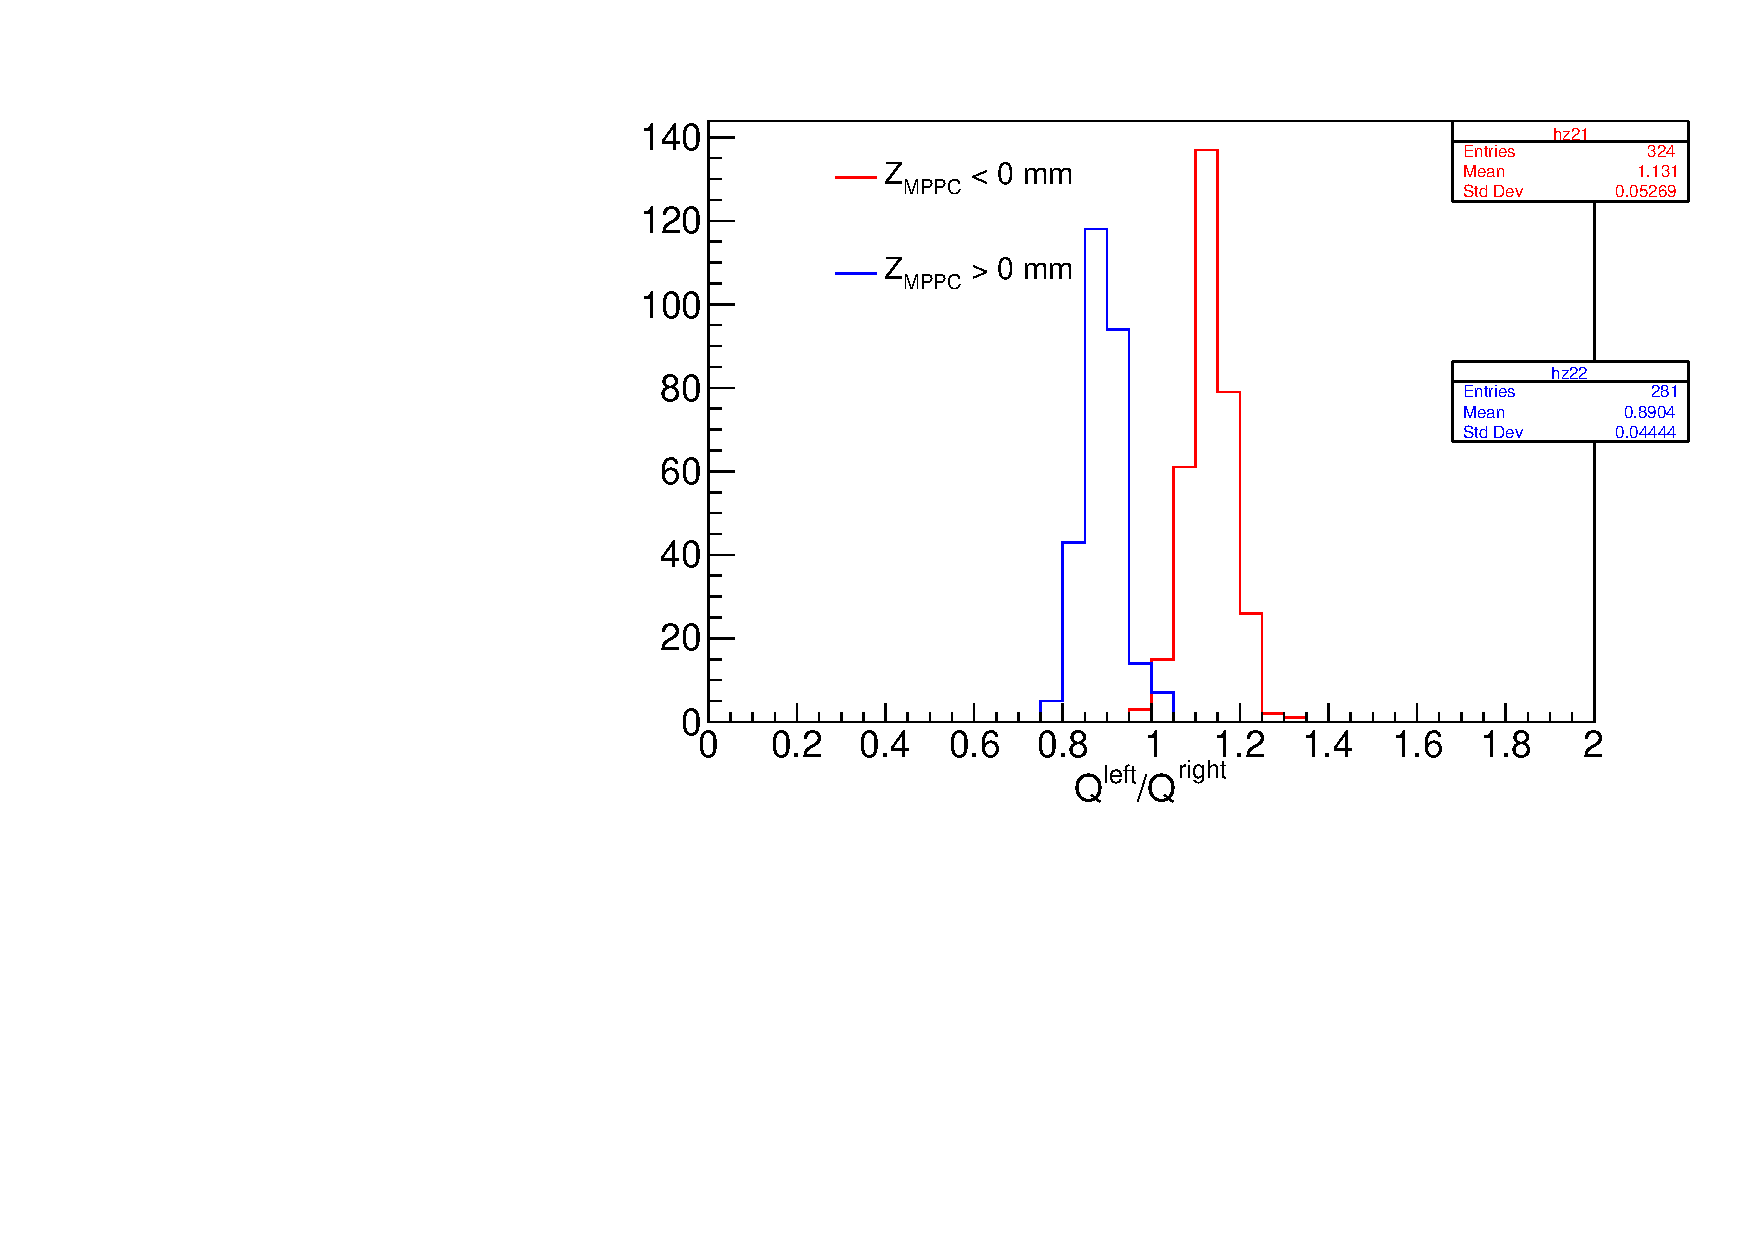
\includegraphics[width=4cm]{plots/2018/h1_z.pdf}
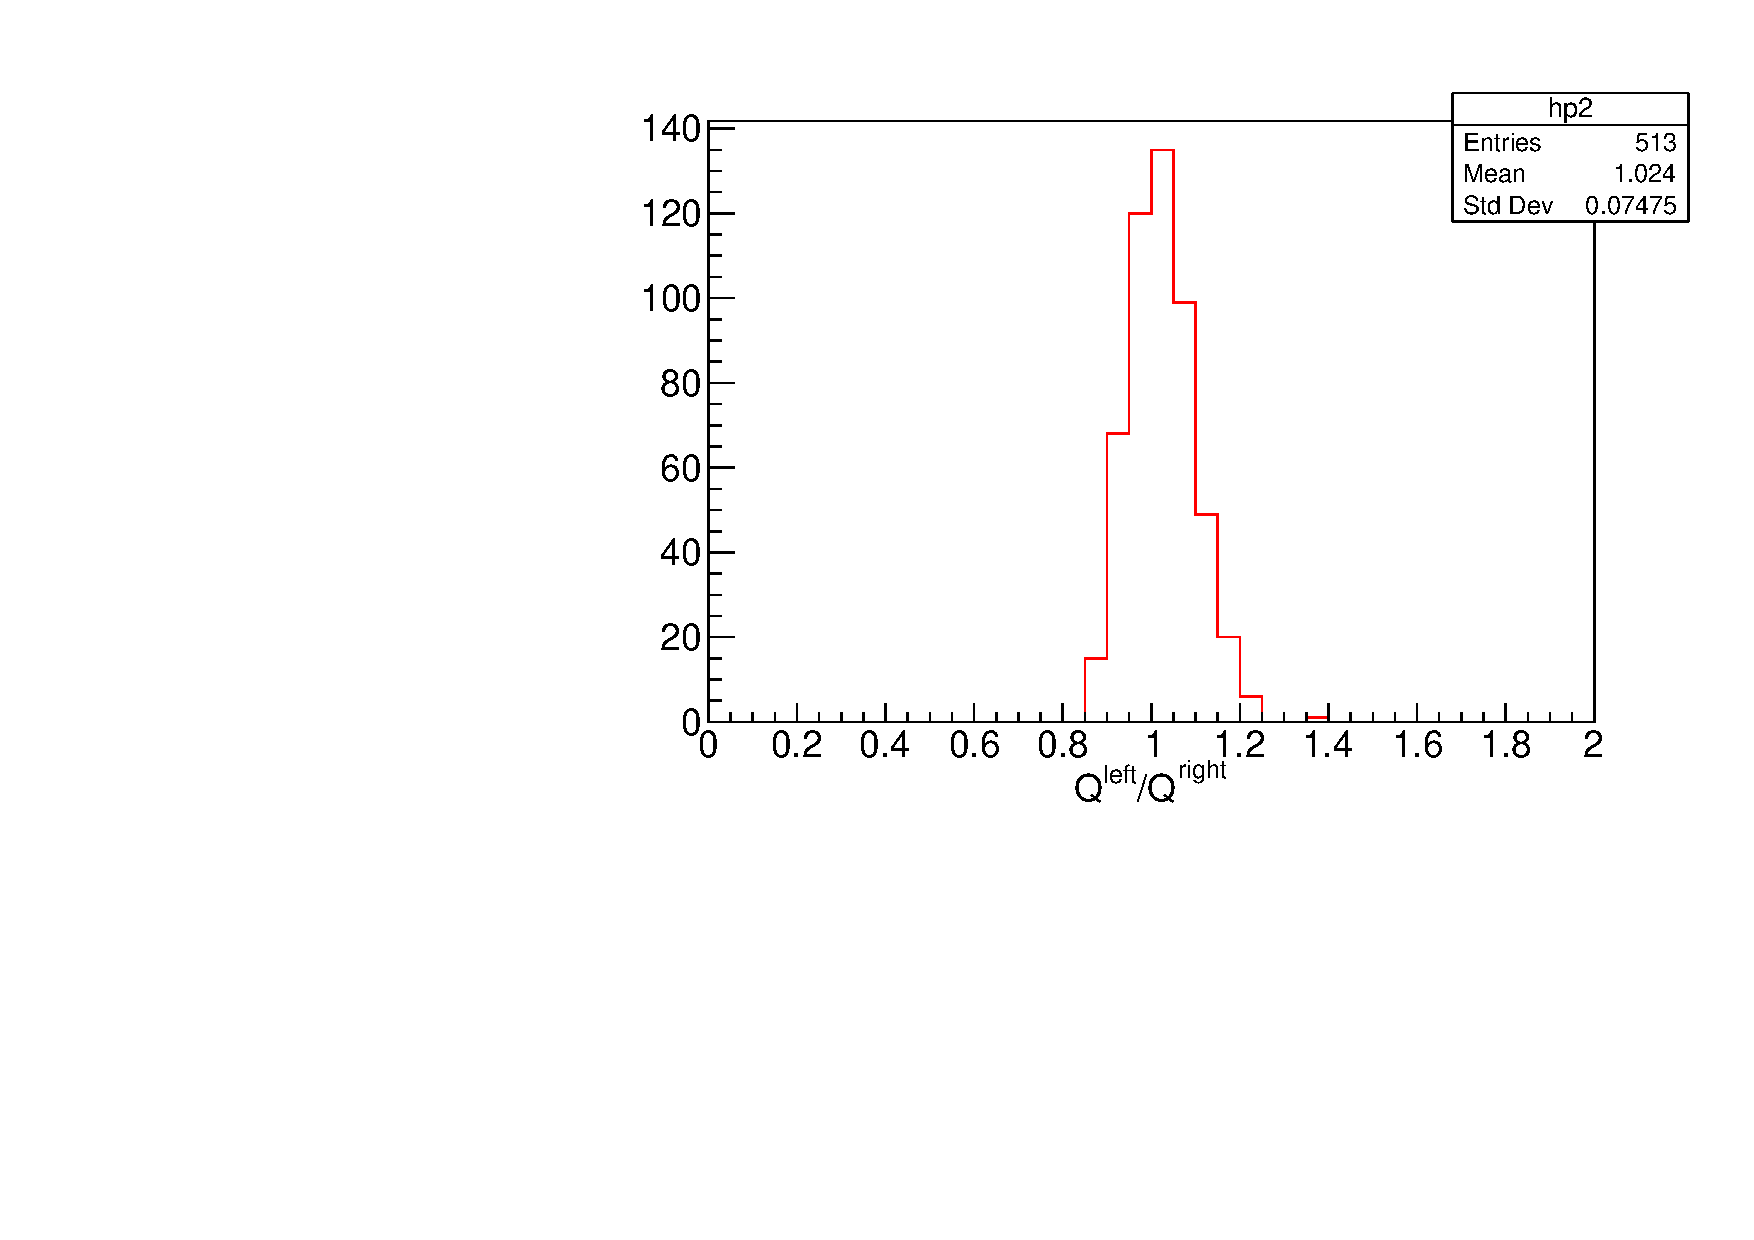
\includegraphics[width=4cm]{plots/2018/h1_phi.pdf}
\caption{Relative mean charge in positive and negative half of the 
photodetectors in z and \phis scans.}
\label{fig:pixelcharge} 
\end{figure}



